% ----------------------------------------------------------------------

\newpage

\subsection{\trimming Test}
\label{ss:trimming}

\subsubsection{Purpose}

The \trimming test accounts for variations in the sensitivities of the 4,160 PUCs within a \roc.
By using the combined effect of the \vthrcomp, \vtrim, and the \trimbits,
it attempts to calibrate every PUC to the same threshold in terms of the calibration pulse strength.
These \dacs can be seen in Figure~\ref{fig:puc} as inputs into the ``trimming'' and ``comparator'' elements of the PUC.
\vtrim sets a coarse scale for the trimming and the \trimbits further fine tune the trimming.
While \vthrcomp and \vtrim are \roc-wide values, there exist four \trimbits for every pixel in a \roc.
``Trimming'' a \roc using \vtrim and the \trimbits effectively means reducing the signal amplitude required to fire the comparator.
Once a module is trimmed, all pixels should turn on at a user-defined threshold (default is \vcal = 35 (low range)).
Thus, input signals with less strength than this threshold will not fire the comparator and will not be registered as a hit.
This ensures that all pixels within a module have a uniform level of zero-suppression.
Additionally, the \trimbit subtest verifies that all trim bits are working
by sequentially enabling each bit and observing its effect on the
pixel threshold distribution (there is not much added benefit of this
test once a ROC has been trimmed successfully---which would not be
possible with defective trim bits). 

\subsubsection{Methodology}

It is important to understand the relevant \dacs for this test: \vthrcomp, \vtrim, and the \trimbits.
\vthrcomp sets a baseline threshold for the comparator unit.
This threshold can be reduced (i.e. ``trimmed'') through the combined effect of \vtrim and the \trimbits.
\vtrim sets the \roc-wide scale for the effect of the \trimbits.
Hence, it can be thought of as a multiplicative factor being applied to the \trimbits.
It is important to note that a trim bit is ``enabled'' when set to zero, 
such that all bits are active when \trimbits=0 [0000] and all bits are inactive when \trimbits=15 [1111].
Thus, the combined effect of \vtrim and the \trimbits is proportional to \vtrim$\times$(15-\trimbits).
The trimming is effectively turned off when either \vtrim=0 or when \trimbits=15.
\\\\
The \trimming test is made up of two subtests: the \trim subtest and the \trimbit subtest. 
The \trim test sets \vthrcomp, \vtrim, and the \trimbits, while the \trimbit test just validates that each of the \trimbits is functioning.
\\\\
The \trim test is responsible for optimizing three \dacs: \vthrcomp, \vtrim, and the \trimbits.
As with other tests, these \dacs are set independently for each \roc.
The \trim test first optimizies \vthrcomp.
To remove the effect of \vtrim and the \trimbits, \vtrim is initialized to zero.
With \vcal set to the target threshold (default is 35), it produces s-curves for all pixels with respect to \vthrcomp.
S-curve tests are described in more detail in Section~\ref{ss:scurves}.
From the distribution of turn-on values (Figure~\ref{fig:trim_thr_TrimThr0_vthrcomp}), 
the entry with the lowest \vthrcomp turn-on is chosen and \vthrcomp is set to this value.
In this process, pixels with turn-on values more than 2$\sigma$ below the mean of the distribution are not considered.
At this \vthrcomp value, all pixels should turn on at \vcal values higher than the target value.
This is because the effect of \vtrim and the \trimbits is to reduce the threshold of the comparator.
Therefore, with \vcal set to the target value, none of pixels should be firing with \vtrim set to zero.
Furthermore, this minimum \vthrcomp value is required to be at least 10 \dac units 
below the \vthrcomp turn-off value for the pixel with the smallest \vthrcomp turn-off.
This ensures none of the pixels could potentially fire on noise at this \vthrcomp value.
\\\\
With an optimal setting for \vthrcomp, the test targets the optimization of \vtrim.
The effect of the \trimbits on the lowering of the comparator threshold is multiplied by the value of \vtrim.
\vtrim should be set to the lowest value that still allows all pixels in the \roc to be successfully trimmed to the target value.
In this way, the entire 4-bit range of the \trimbits is used, maximizing the precision of the trimming.
Setting \vtrim any higher than this would just compress the range of the \trimbits used.
To find the minimal effective value of \vtrim, the test first identifies the pixel with the highest \vcal turn-on, 
using the standard s-curve procedure (Figure~\ref{fig:trim_thr_TrimThr1_vcal}).
This is the pixel that requires the most trimming to have its \vcal threshold reduced to the target value.
The test then enables all four \trimbits (\trimbits=0), maximizing their effect.
Using this pixel, the test performs an efficiency scan over the \vtrim and \vcal~\dacs (Figure~\ref{fig:trim_trim_VCAL_VTRIM}).
Starting at high \vtrim, the value of \vtrim is iteratively lowered until the \vcal turn-on surpasses the target \vcal.
This value of \vtrim corresponds to the minimum value that can effectively trim this pixel, 
and it is chosen as the final \vtrim value for the \roc.
This procedure effectively sets the level of \vtrim at which the chosen pixel needs all four bits enabled to be trimmed.
Since this pixel is known to need the most trimming, 
all other pixels can by definition be trimmed with an equal or lesser number of trim bits enabled.
\\\\
With the appropriate dynamic range for the trimming set using \vthrcomp and \vtrim, 
the test can proceed to fine tune the trimming for each individual pixel using the four \trimbits.
This is achieved using a binary search tree algorithm.
Starting with the \trimbits set to 7 [0111] (in the center of their 0-15 range), 
\vcal turn-on thresholds are determined via s-curves (Figure~\ref{fig:trim_thr_TrimThr2_vcal}).
For any pixel that fires below (above) the target \vcal value, the \trimbits value is increased (decreased) by 4, 
so that the amount of trimming is decreased (increased).
The s-curve test is repeated (Figure~\ref{fig:trim_thr_trimStepCorr4_vcal}), and the \trimbits values are increased or decreased by 2, as appropriate.
The procedure is repeated two more times (Figures~\ref{fig:trim_thr_trimStepCorr2_vcal},~\ref{fig:trim_thr_trimStepCorr1a_vcal}), with an increment of one, 
so that all possible values of the \trimbits are within reach of the test.
The turn-on thresholds after the final correction are shown in Figure~\ref{fig:trim_thr_trimStepCorr1b_vcal}.
The optimized values of the \trimbits are shown in Figures~\ref{fig:trim_TrimMap} and~\ref{fig:trim_dist_TrimMap}.
To validate that the trimming was reasonably effective, 
a final s-curve test is performed (Figures~\ref{fig:trim_thr_TrimThrFinal_vcal},~\ref{fig:trim_dist_thr_TrimThrFinal_vcal}).
\\\\
The \trimbit test verifies that all \trimbits are programmable.
Since (in conjunction with \vtrim) the \trimbits alter the threshold of the comparator,
enabling a given bit should have a measurable effect on the \vcal turn-on for the pixel in question.
\vtrim is set to the minimum value (0),
and s-curves (with respect to \vcal) are obtained with all \trimbits disabled (\trimbits=15 [1111]).
The turn-on values extracted from these curves serve as untrimmed baseline values (Figure~\ref{fig:trim_thr_TrimBitsThr0_Vcal}).
Then each bit is enabled in turn and new s-curves are recorded for values of 
\trimbits=14 [1110] (Figure~\ref{fig:trim_thr_TrimThr_trim14_Vcal}),
\trimbits=13 [1101] (Figure~\ref{fig:trim_thr_TrimThr_trim13_Vcal}),
\trimbits=11 [1011] (Figure~\ref{fig:trim_thr_TrimThr_trim11_Vcal}), 
and \trimbits=7 [0111] (Figure~\ref{fig:trim_thr_TrimThr_trim7_Vcal}).
At each iteration, \vtrim is reduced by a factor of (roughly) two to cancel out the effect of which bit is being enabled.
Then each set of turn-on values is subtracted from the baseline set, to isolate the effect of enabling a single trim bit.
Distributions of these differences are shown for 
\trimbits=14 [1110] (Figure~\ref{fig:trim_TrimBit14}),
\trimbits=13 [1101] (Figure~\ref{fig:trim_TrimBit13}),
\trimbits=11 [1011] (Figure~\ref{fig:trim_TrimBit11}),
and \trimbits=7 [0111] (Figure~\ref{fig:trim_TrimBit7}).
If the difference is larger than zero, the trim bit in question is programmable and is having a noticeable effect.
Pixels with a defective trim bit are flagged.

\subsubsection{Output}

\begin{figure}[!htp]
\centering
\begin{minipage}{0.45\textwidth}

% from trim test:  scan to get minimal vthrcomp turn-on pixel
  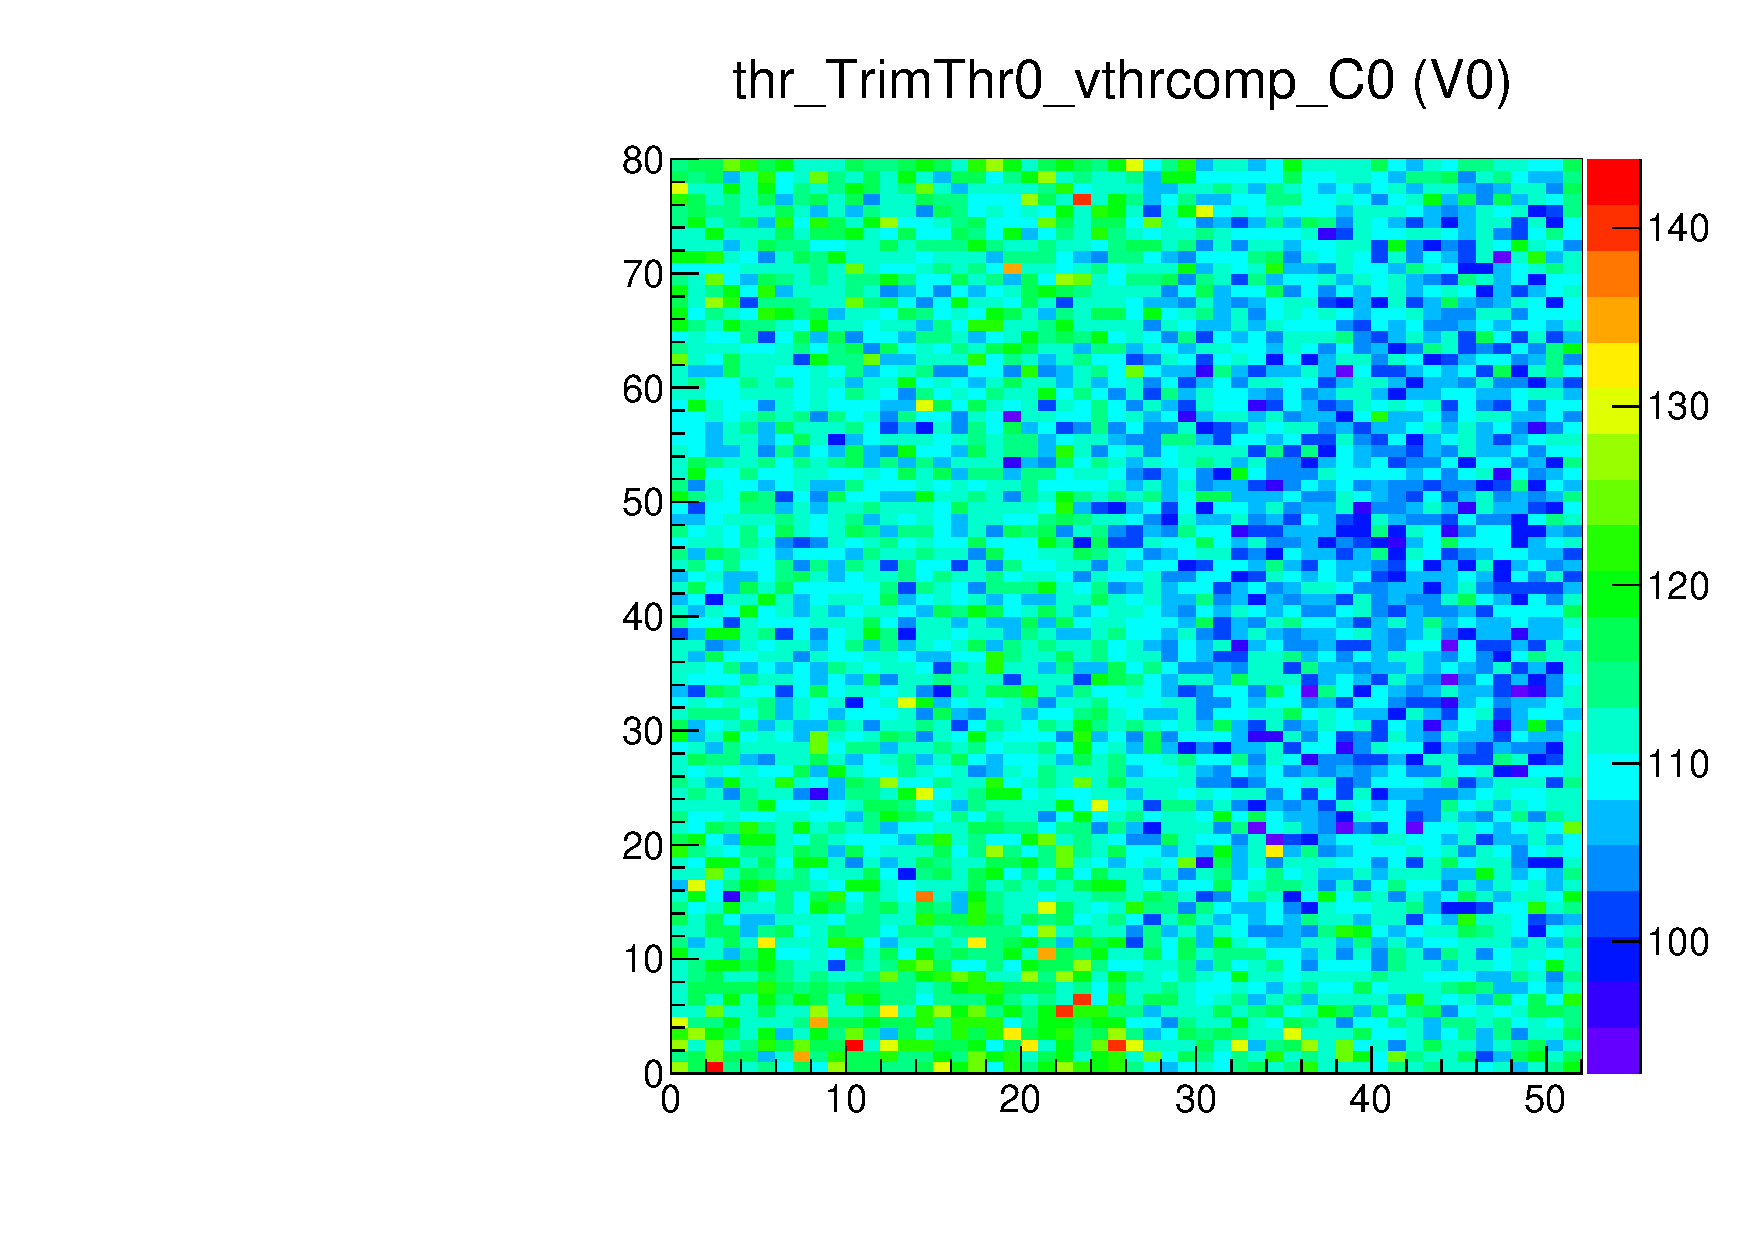
\includegraphics[width=1.0\textwidth]{figures/trim_thr_TrimThr0_vthrcomp.pdf}
  \caption{\roc map of \vthrcomp turn-on thresholds with \vcal set to target value.
           Used to find pixel with minimum turn-on (least sensitive pixel).}
  \label{fig:trim_thr_TrimThr0_vthrcomp}
\end{minipage}
\hspace{0.3cm}
\begin{minipage}{0.45\textwidth}

% from trim test:  scan to get maximal vcal turn-on pixel
  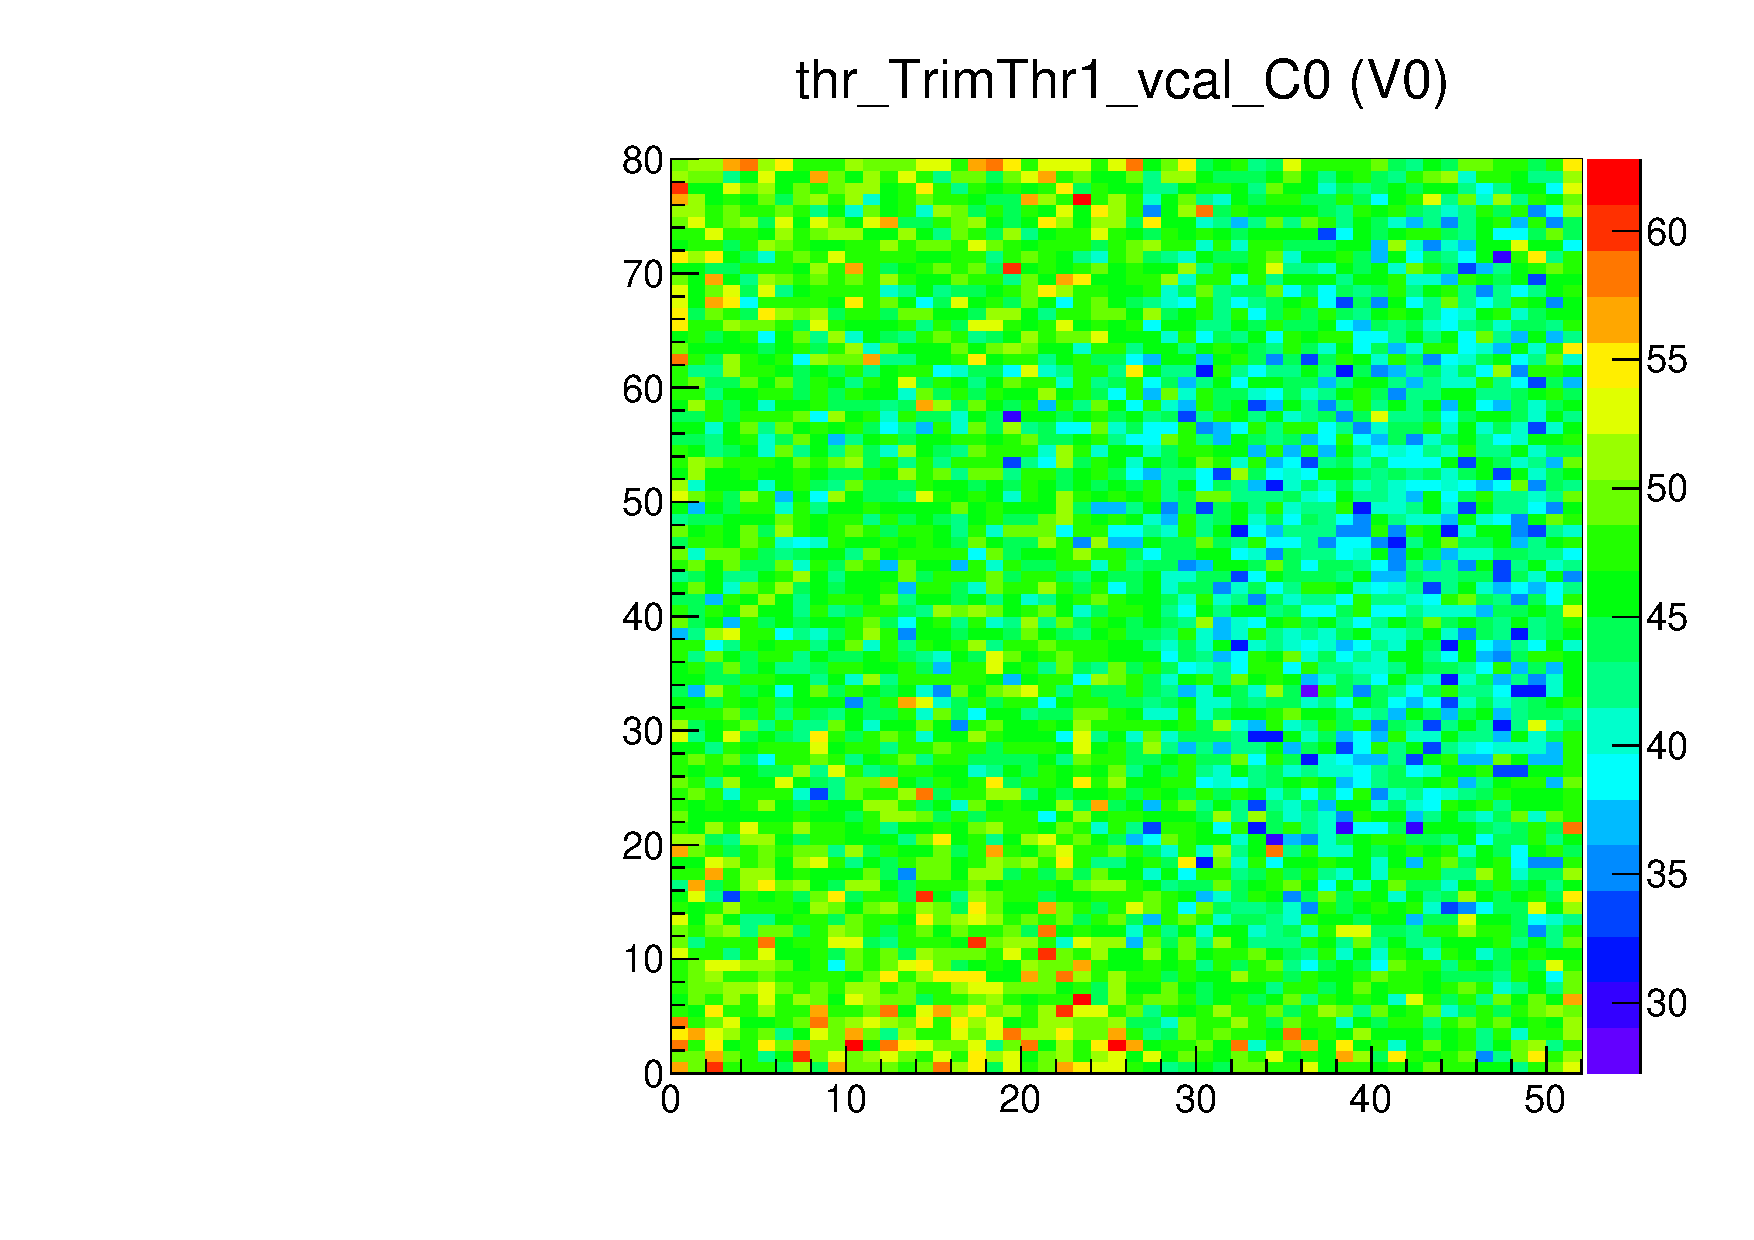
\includegraphics[width=1.0\textwidth]{figures/trim_thr_TrimThr1_vcal.pdf}
  \caption{\roc map of \vcal turn-on thresholds with minimized \vthrcomp value.  
           Used to find most sensitive pixel, i.e. the pixel requiring maximum trimming.}
  \label{fig:trim_thr_TrimThr1_vcal}
\end{minipage}
\end{figure}

% from trim test: efficiency in vcal/trim plane, for setting Vtrim

\begin{figure}[!htp]
\centering
\begin{minipage}{0.45\textwidth}
  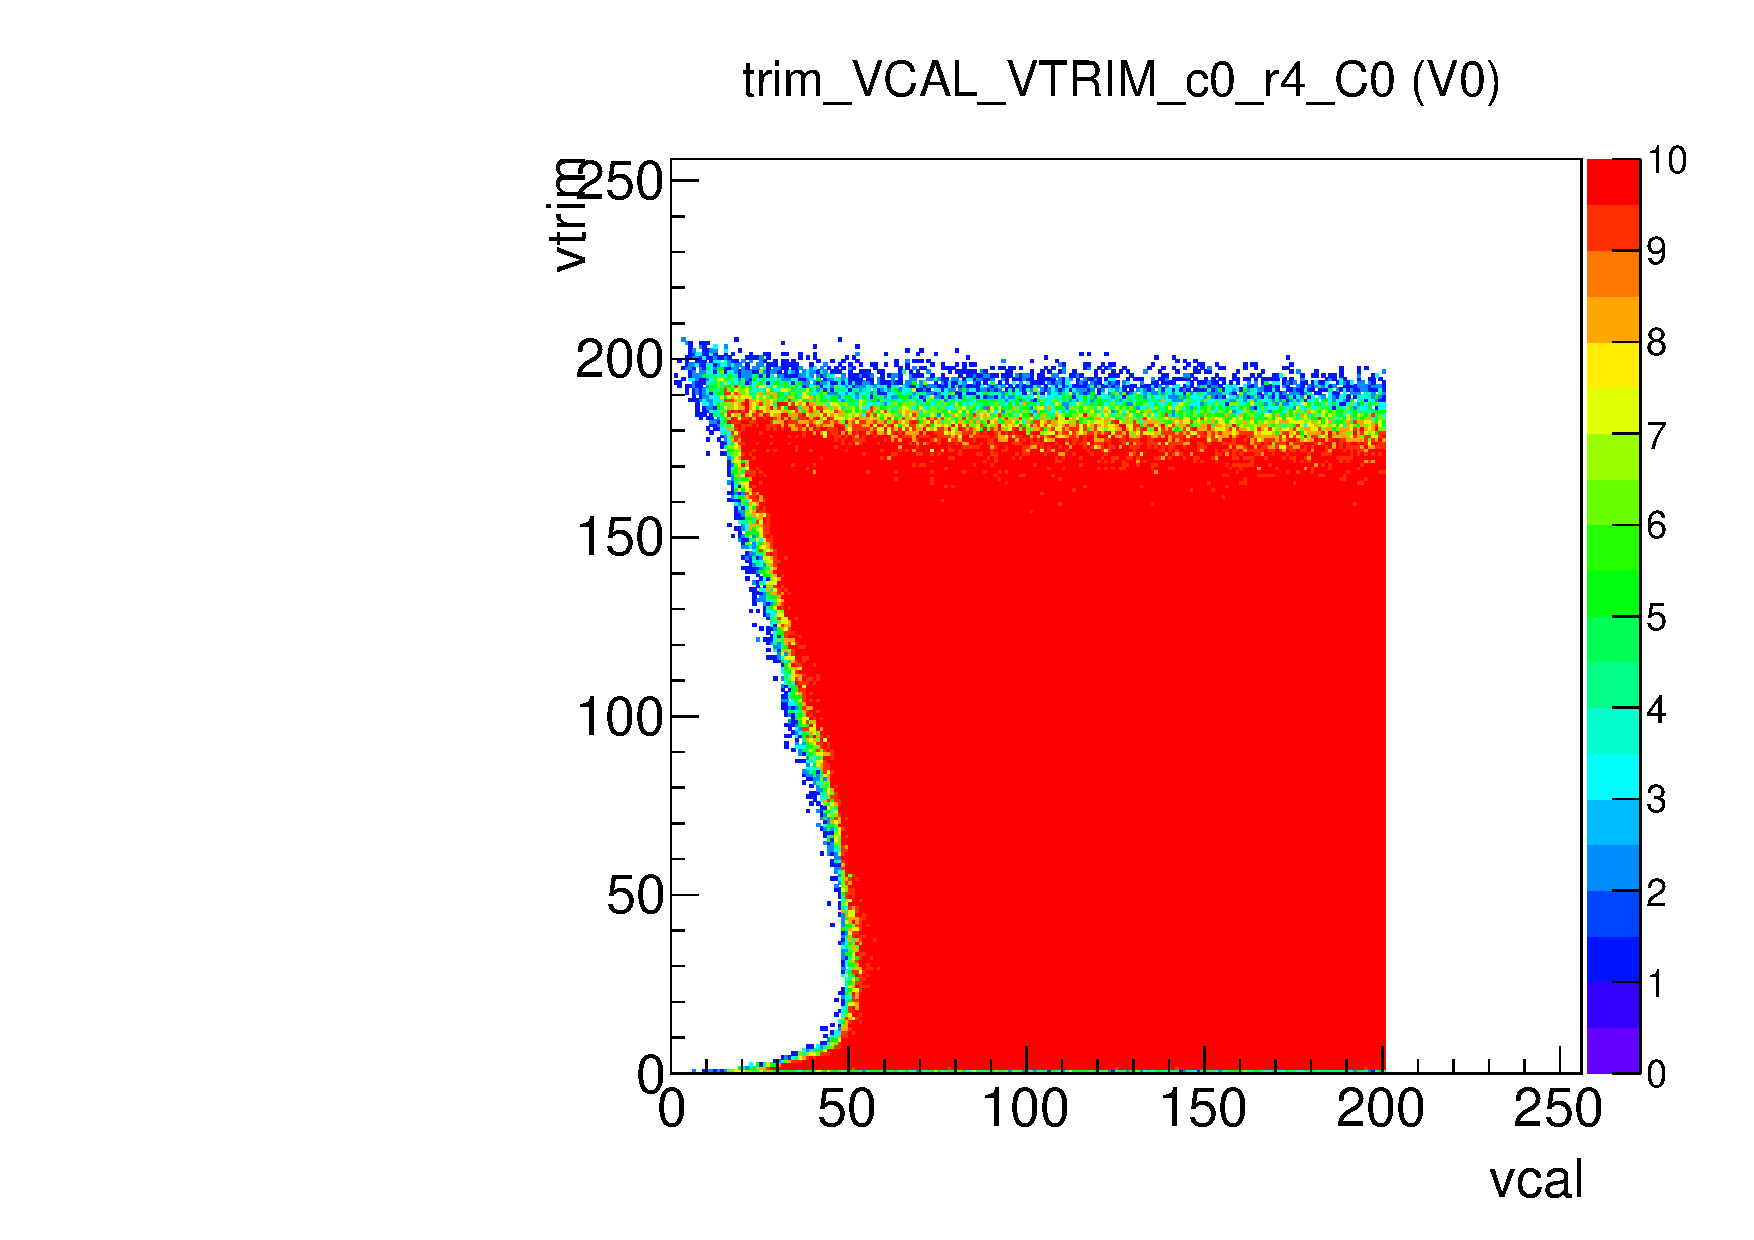
\includegraphics[width=1.0\textwidth]{figures/trim_trim_VCAL_VTRIM.pdf}
  \caption{Efficiency in the \vtrim vs. \vcal plane.
           Used to find the value of \vtrim that corresponds to a turn-on at the target \vcal.}
  \label{fig:trim_trim_VCAL_VTRIM}
\end{minipage}
\end{figure}

% from trim test: threshold maps after each iteration of trim correction

\begin{figure}[!htp]
\centering
\begin{minipage}{0.45\textwidth}
  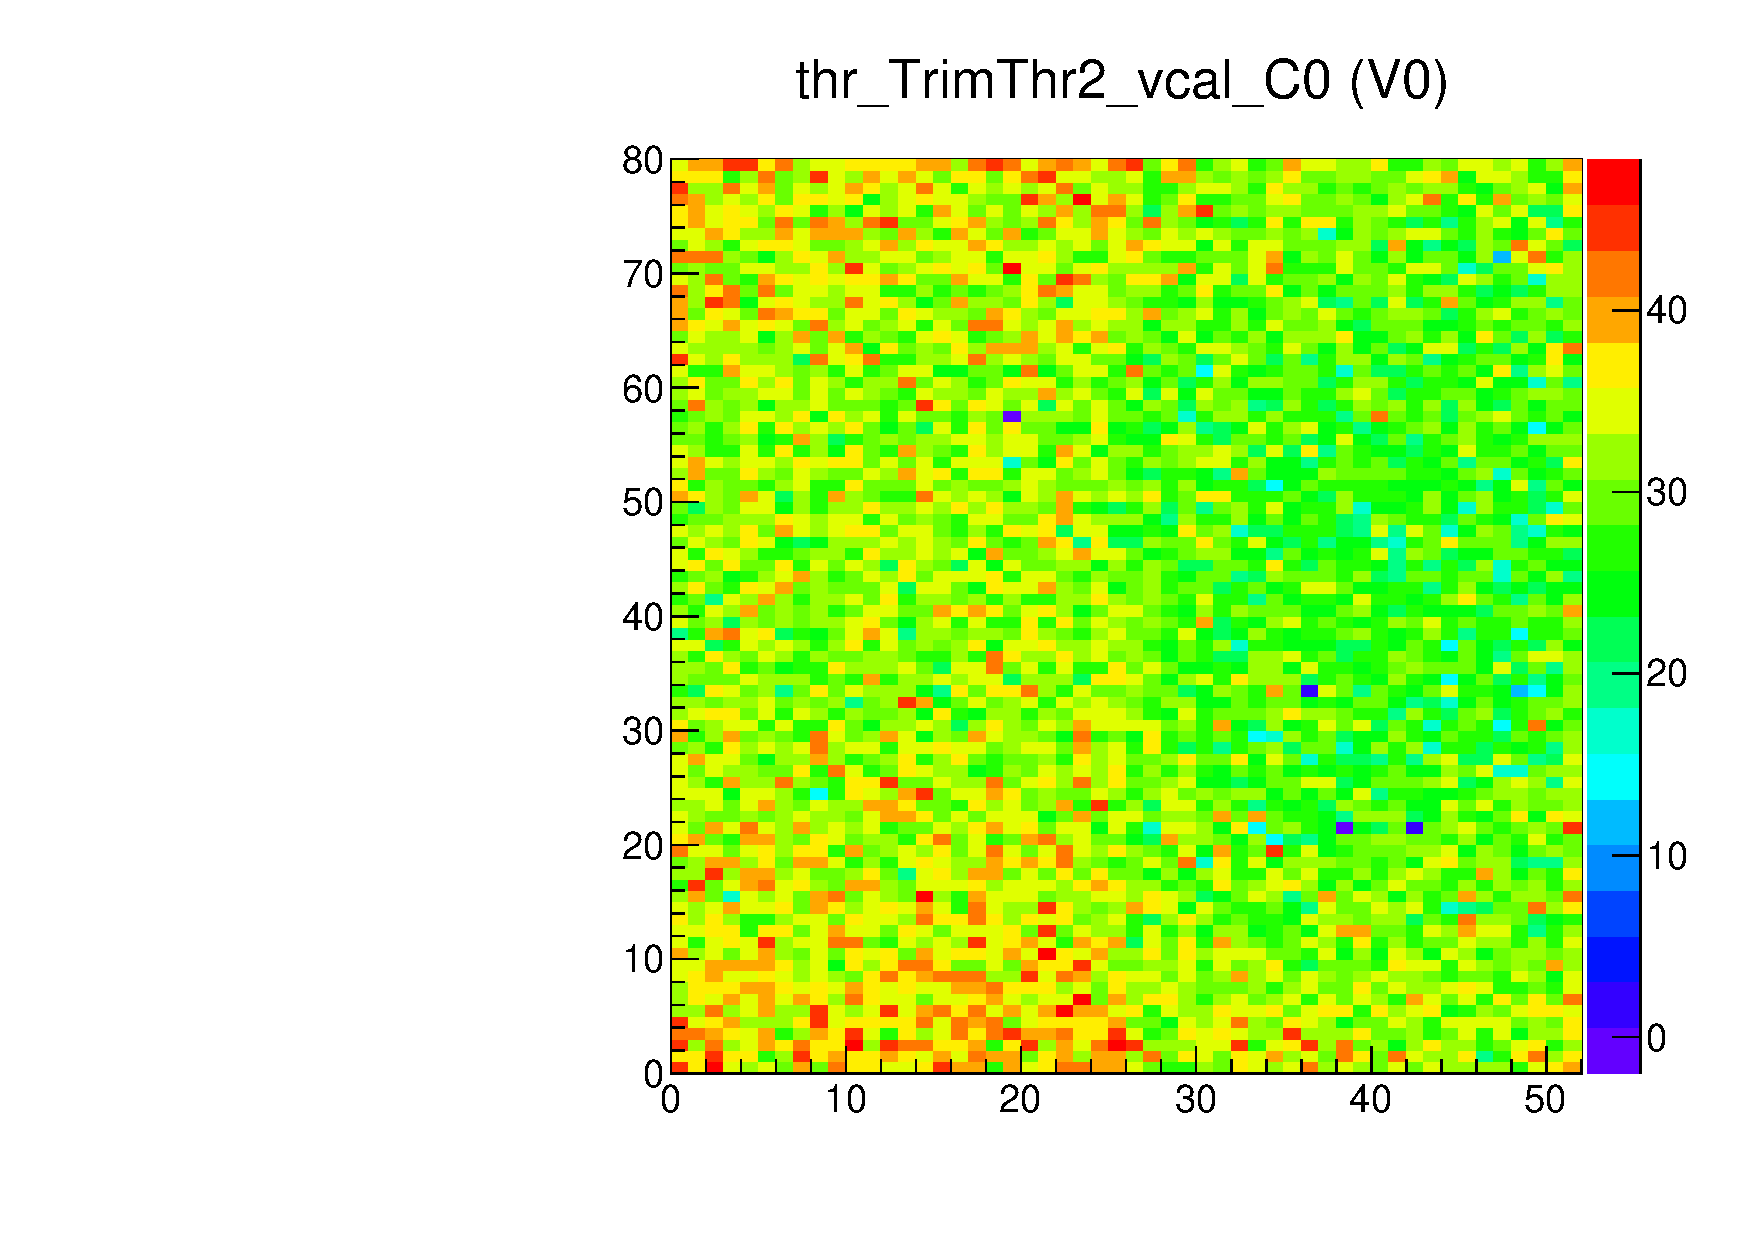
\includegraphics[width=1.0\textwidth]{figures/trim_thr_TrimThr2_vcal.pdf}
  \caption{\roc map of \vcal turn-on thresholds with \trimbits=7.
           Used as baseline for setting the \trimbits.}
  \label{fig:trim_thr_TrimThr2_vcal}
\end{minipage}
\end{figure}

\begin{figure}[!htp]
\centering
\begin{minipage}{0.45\textwidth}
  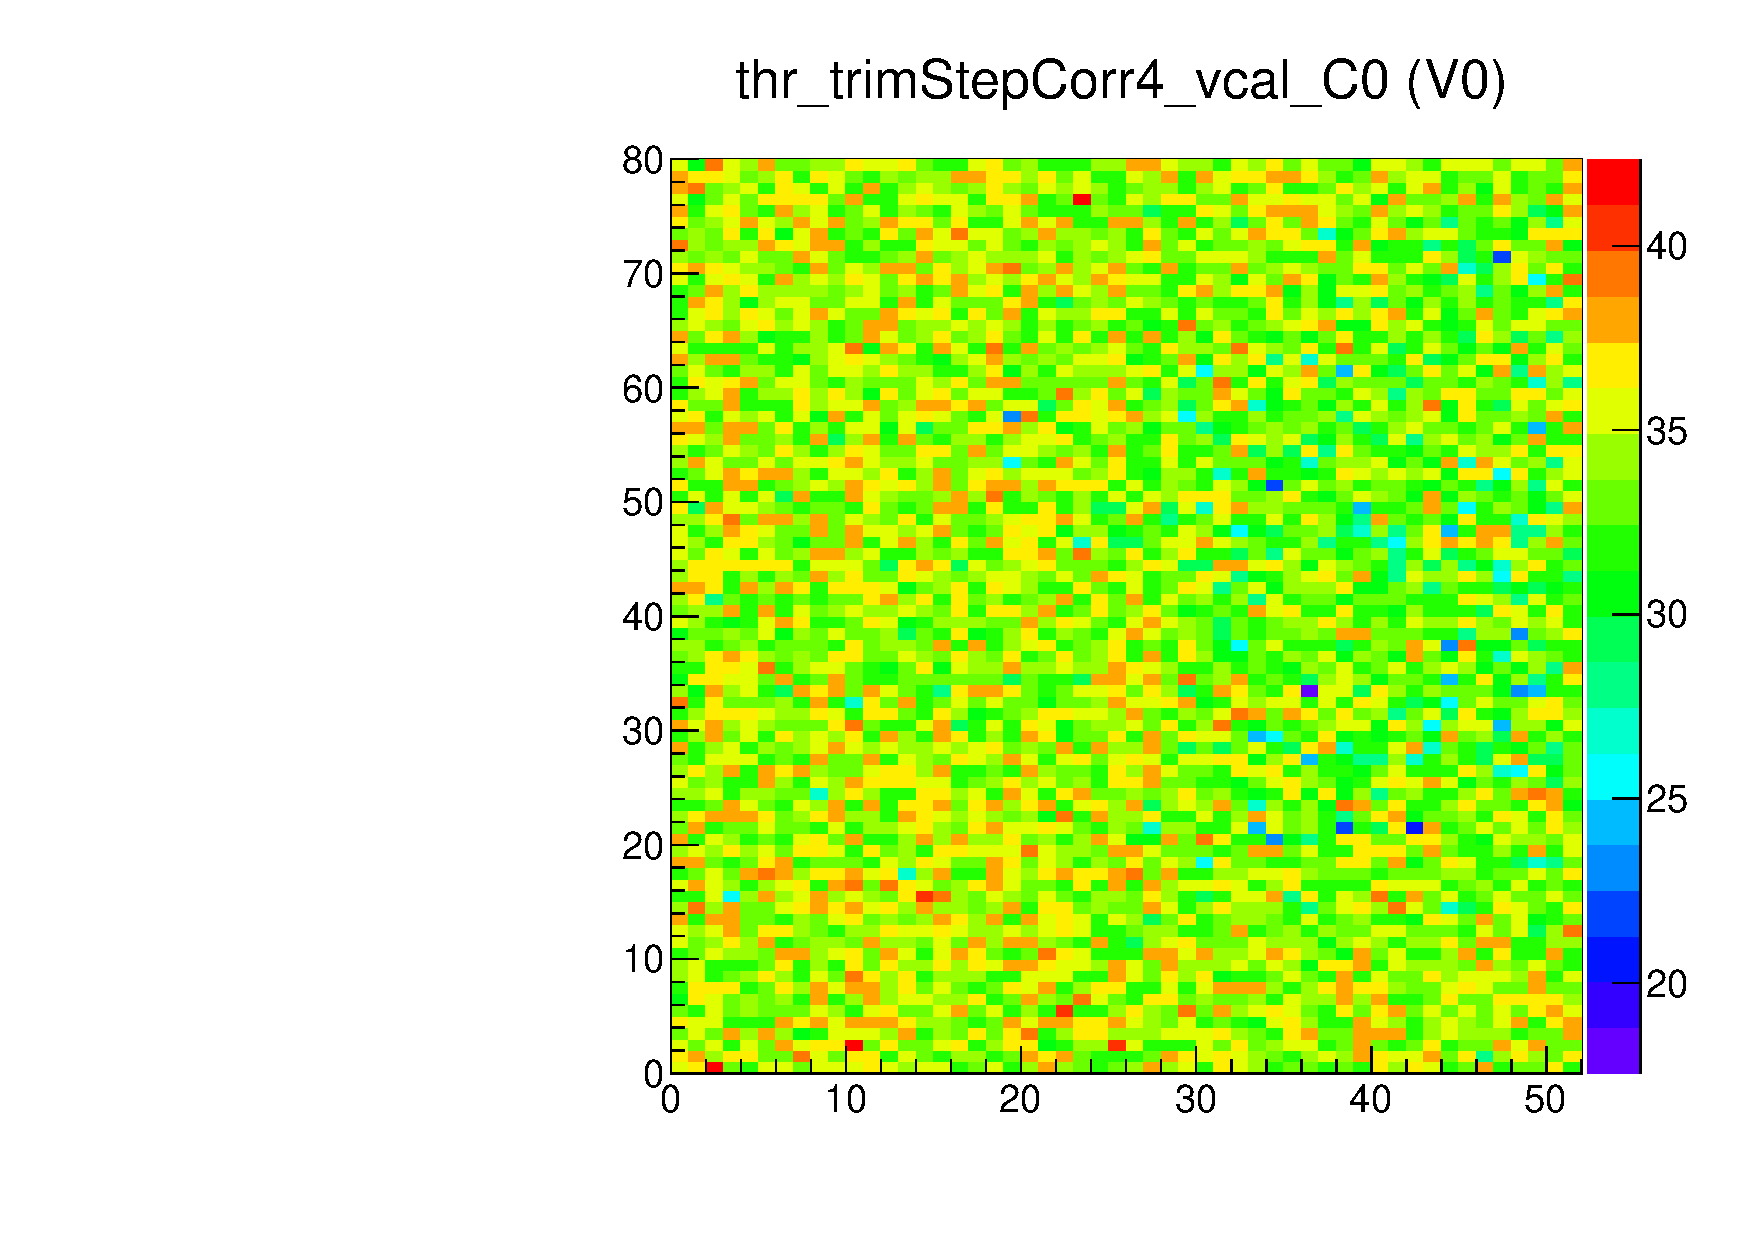
\includegraphics[width=1.0\textwidth]{figures/trim_thr_trimStepCorr4_vcal.pdf}
  \caption{\roc map of \vcal turn-on thresholds after a \trimbits$\pm$4 correction with respect to Figure~\ref{fig:trim_thr_TrimThr2_vcal}.}
  \label{fig:trim_thr_trimStepCorr4_vcal}
\end{minipage}
\hspace{0.3cm}
\begin{minipage}{0.45\textwidth}
  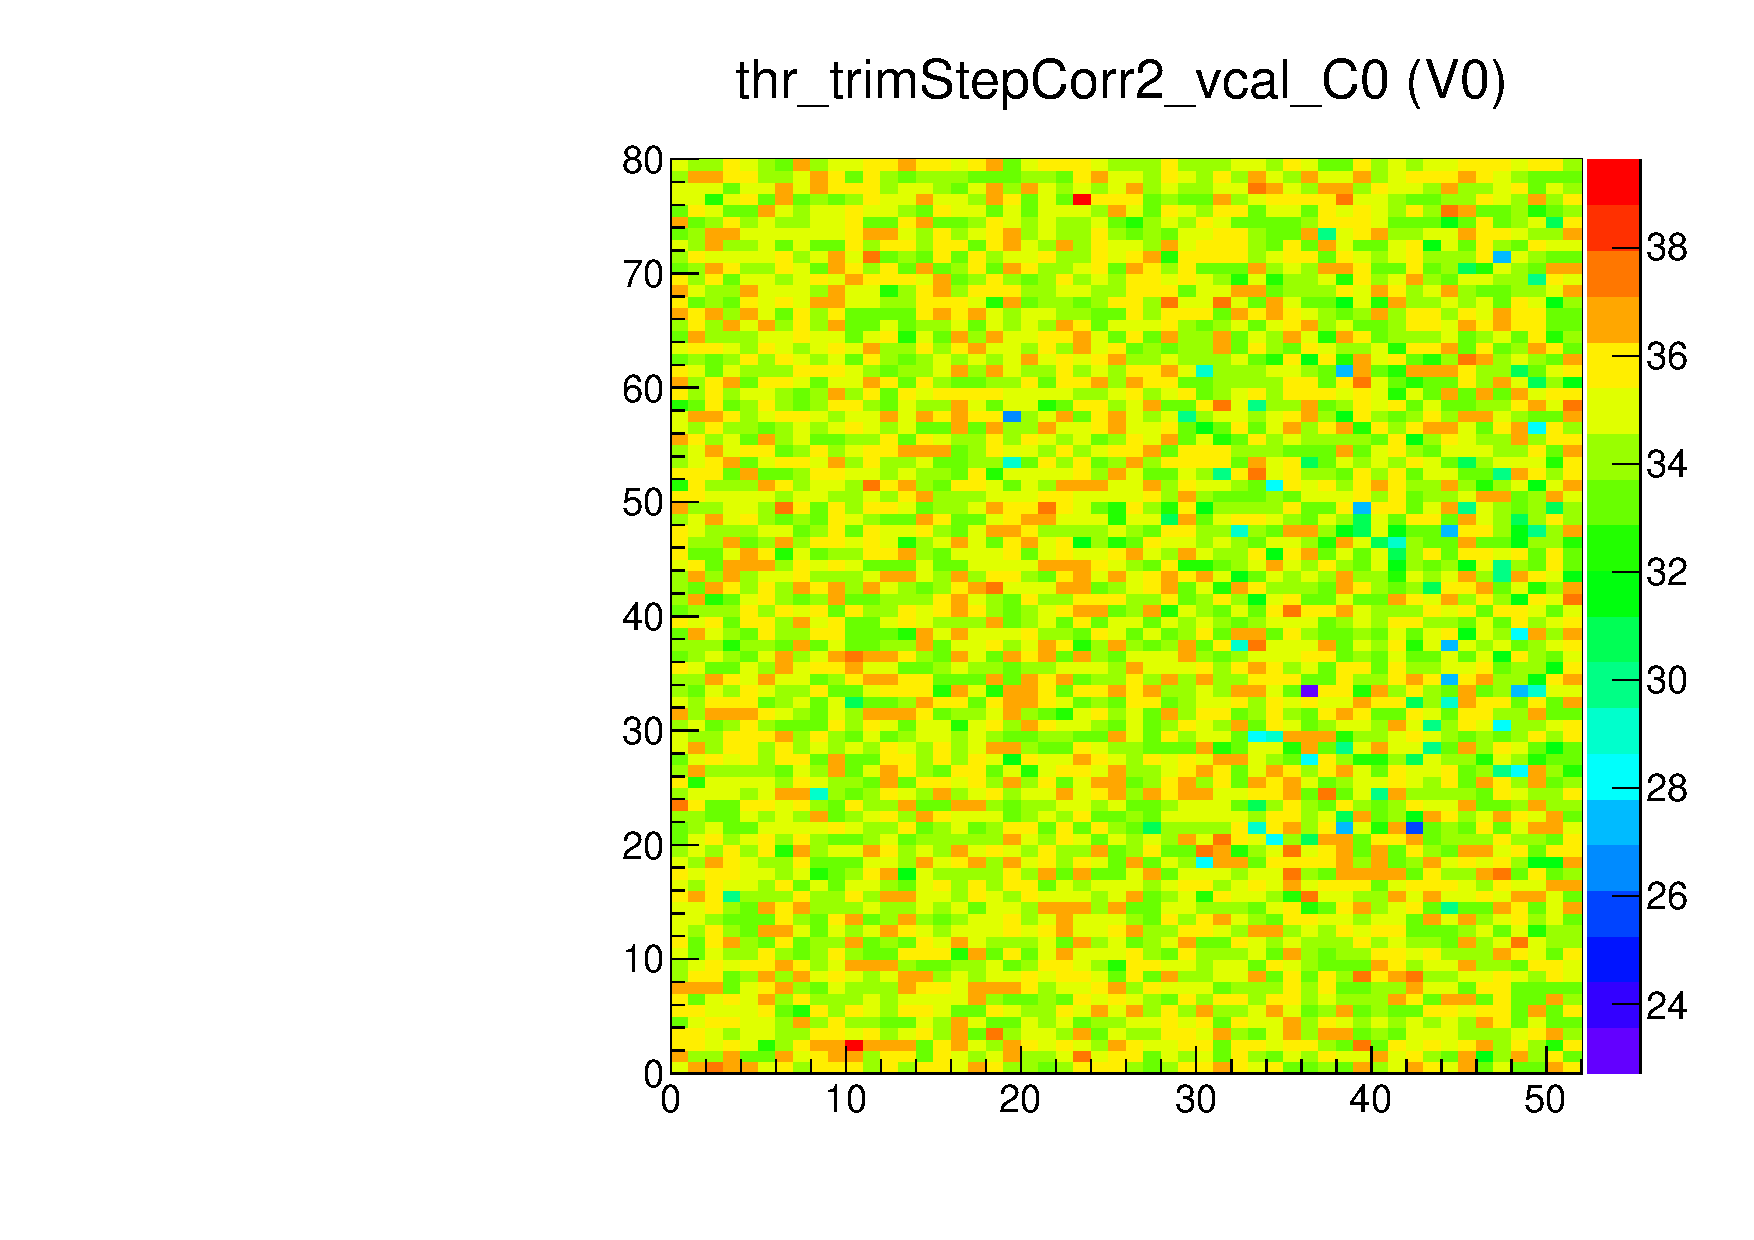
\includegraphics[width=1.0\textwidth]{figures/trim_thr_trimStepCorr2_vcal.pdf}
  \caption{\roc map of \vcal turn-on thresholds after a \trimbits$\pm$2 correction with respect to Figure~\ref{fig:trim_thr_trimStepCorr4_vcal}.}
  \label{fig:trim_thr_trimStepCorr2_vcal}
\end{minipage}
\end{figure}

\begin{figure}[!htp]
\centering
\begin{minipage}{0.45\textwidth}
  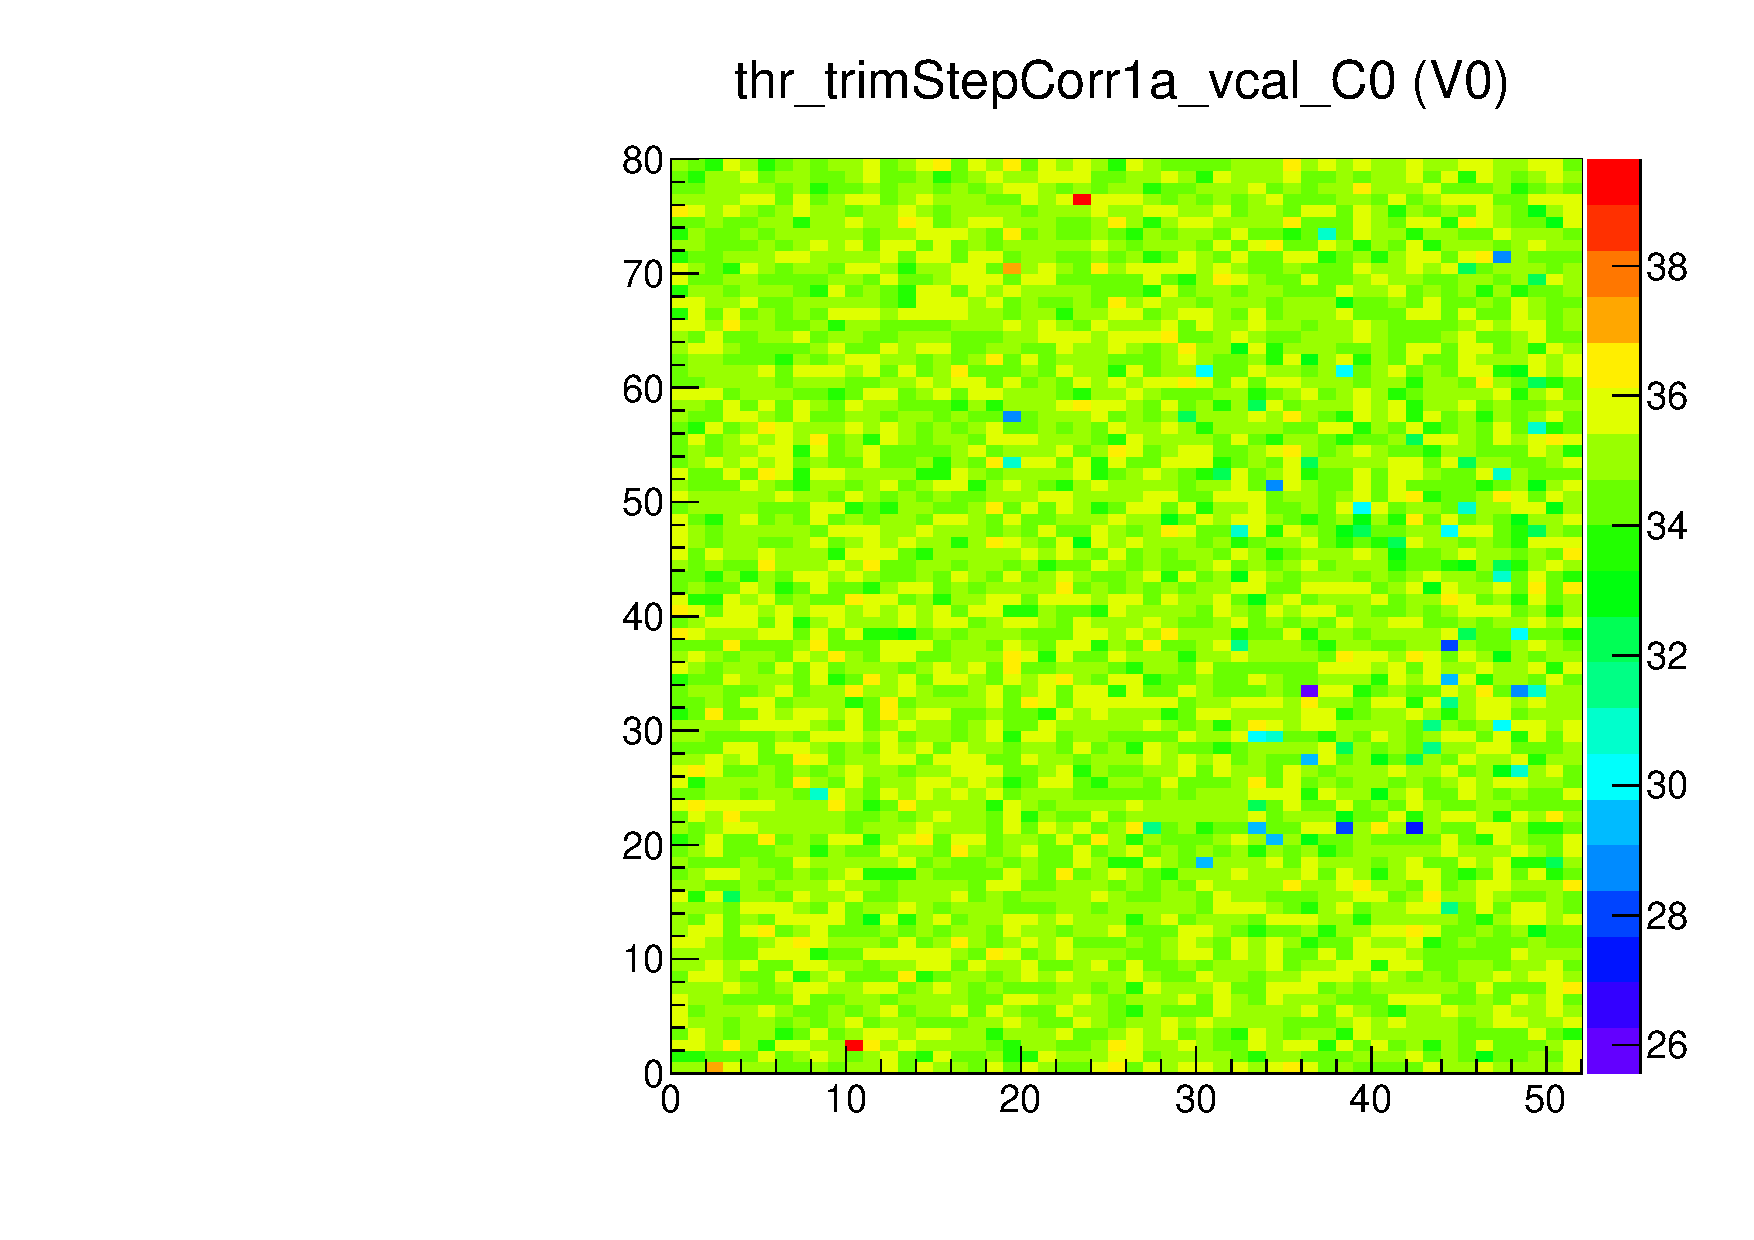
\includegraphics[width=1.0\textwidth]{figures/trim_thr_trimStepCorr1a_vcal.pdf}
  \caption{\roc map of \vcal turn-on thresholds after a \trimbits$\pm$1 correction with respect to Figure~\ref{fig:trim_thr_trimStepCorr2_vcal}.}
  \label{fig:trim_thr_trimStepCorr1a_vcal}
\end{minipage}
\hspace{0.3cm}
\begin{minipage}{0.45\textwidth}
  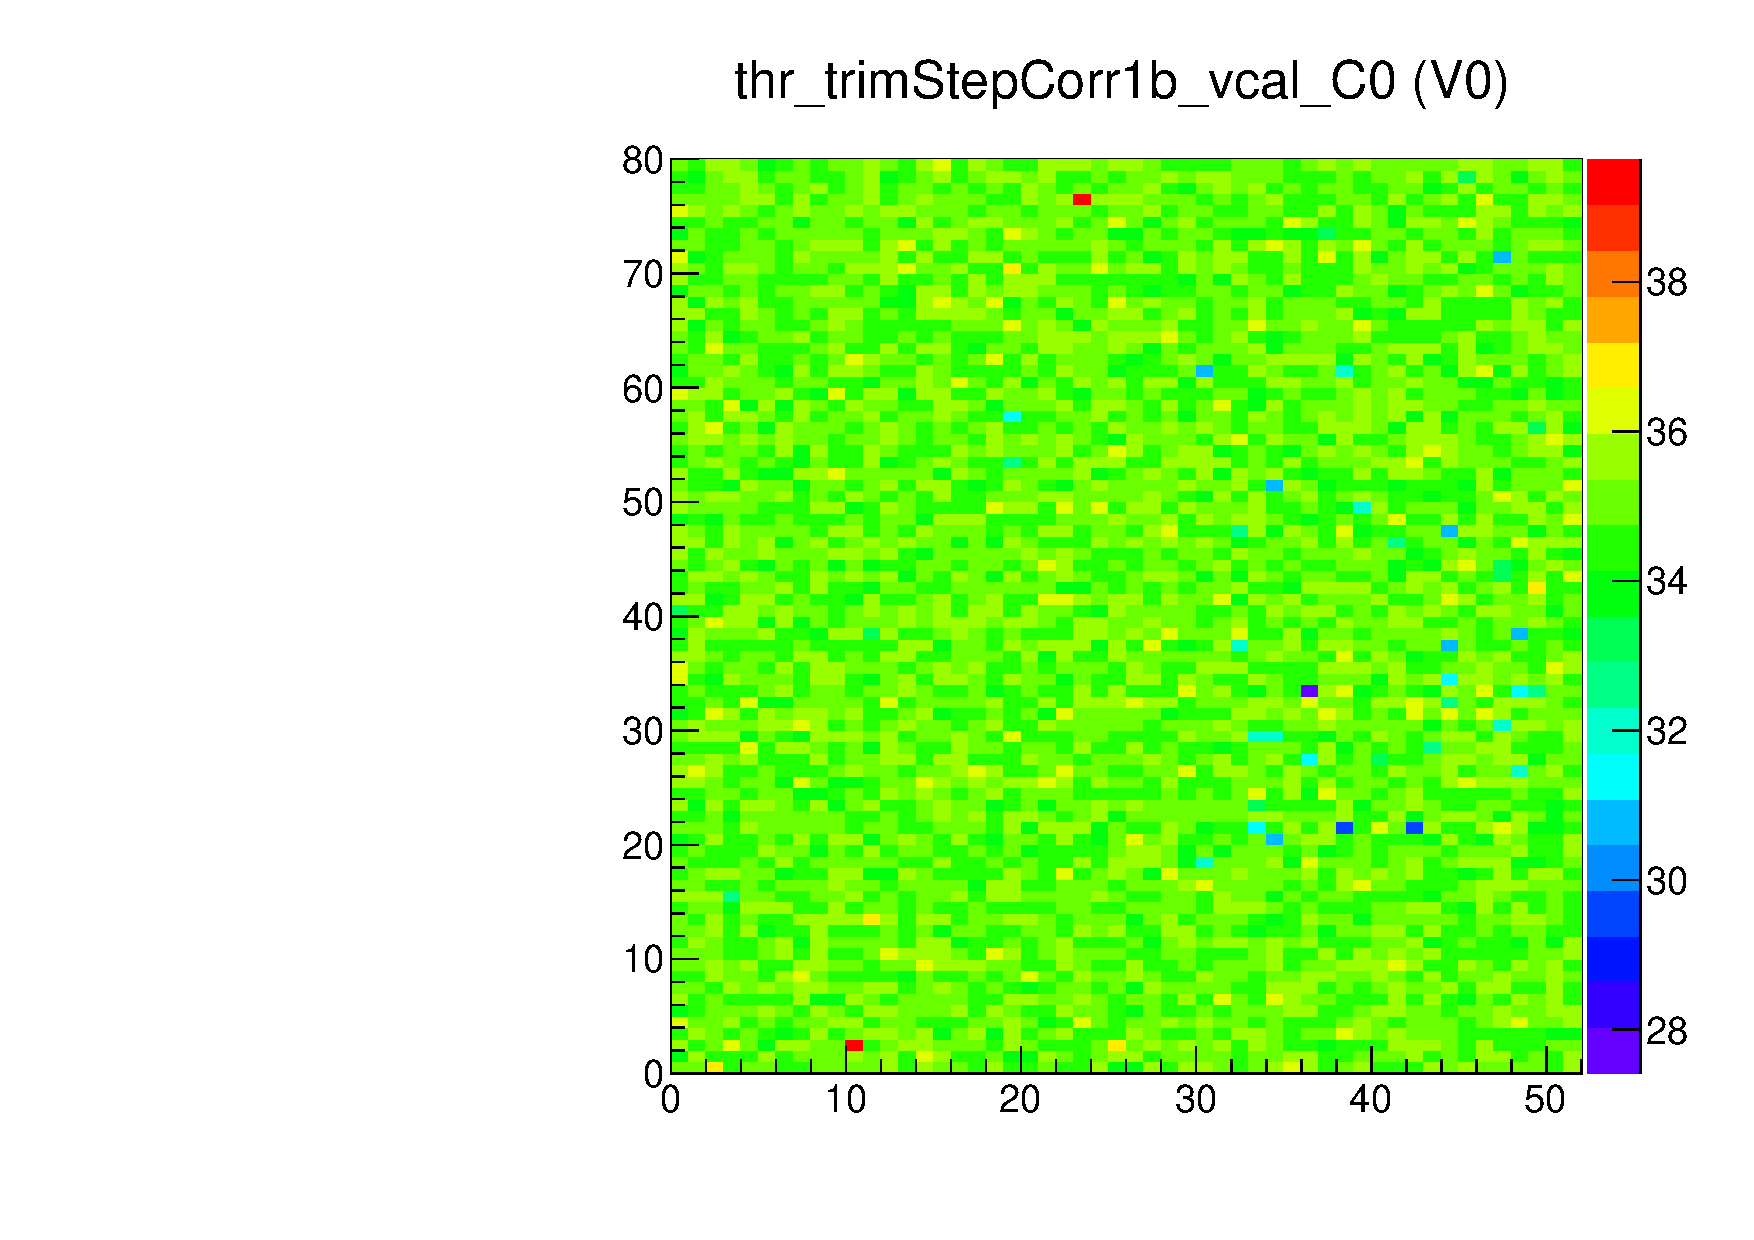
\includegraphics[width=1.0\textwidth]{figures/trim_thr_trimStepCorr1b_vcal.pdf}
  \caption{\roc map of \vcal turn-on thresholds after a \trimbits$\pm$1 correction with respect to Figure~\ref{fig:trim_thr_trimStepCorr1a_vcal}.}
  \label{fig:trim_thr_trimStepCorr1b_vcal}
\end{minipage}
\end{figure}


% from trim test:  optimized trim bits

\begin{figure}[!htp]
\centering
\begin{minipage}{0.45\textwidth}
  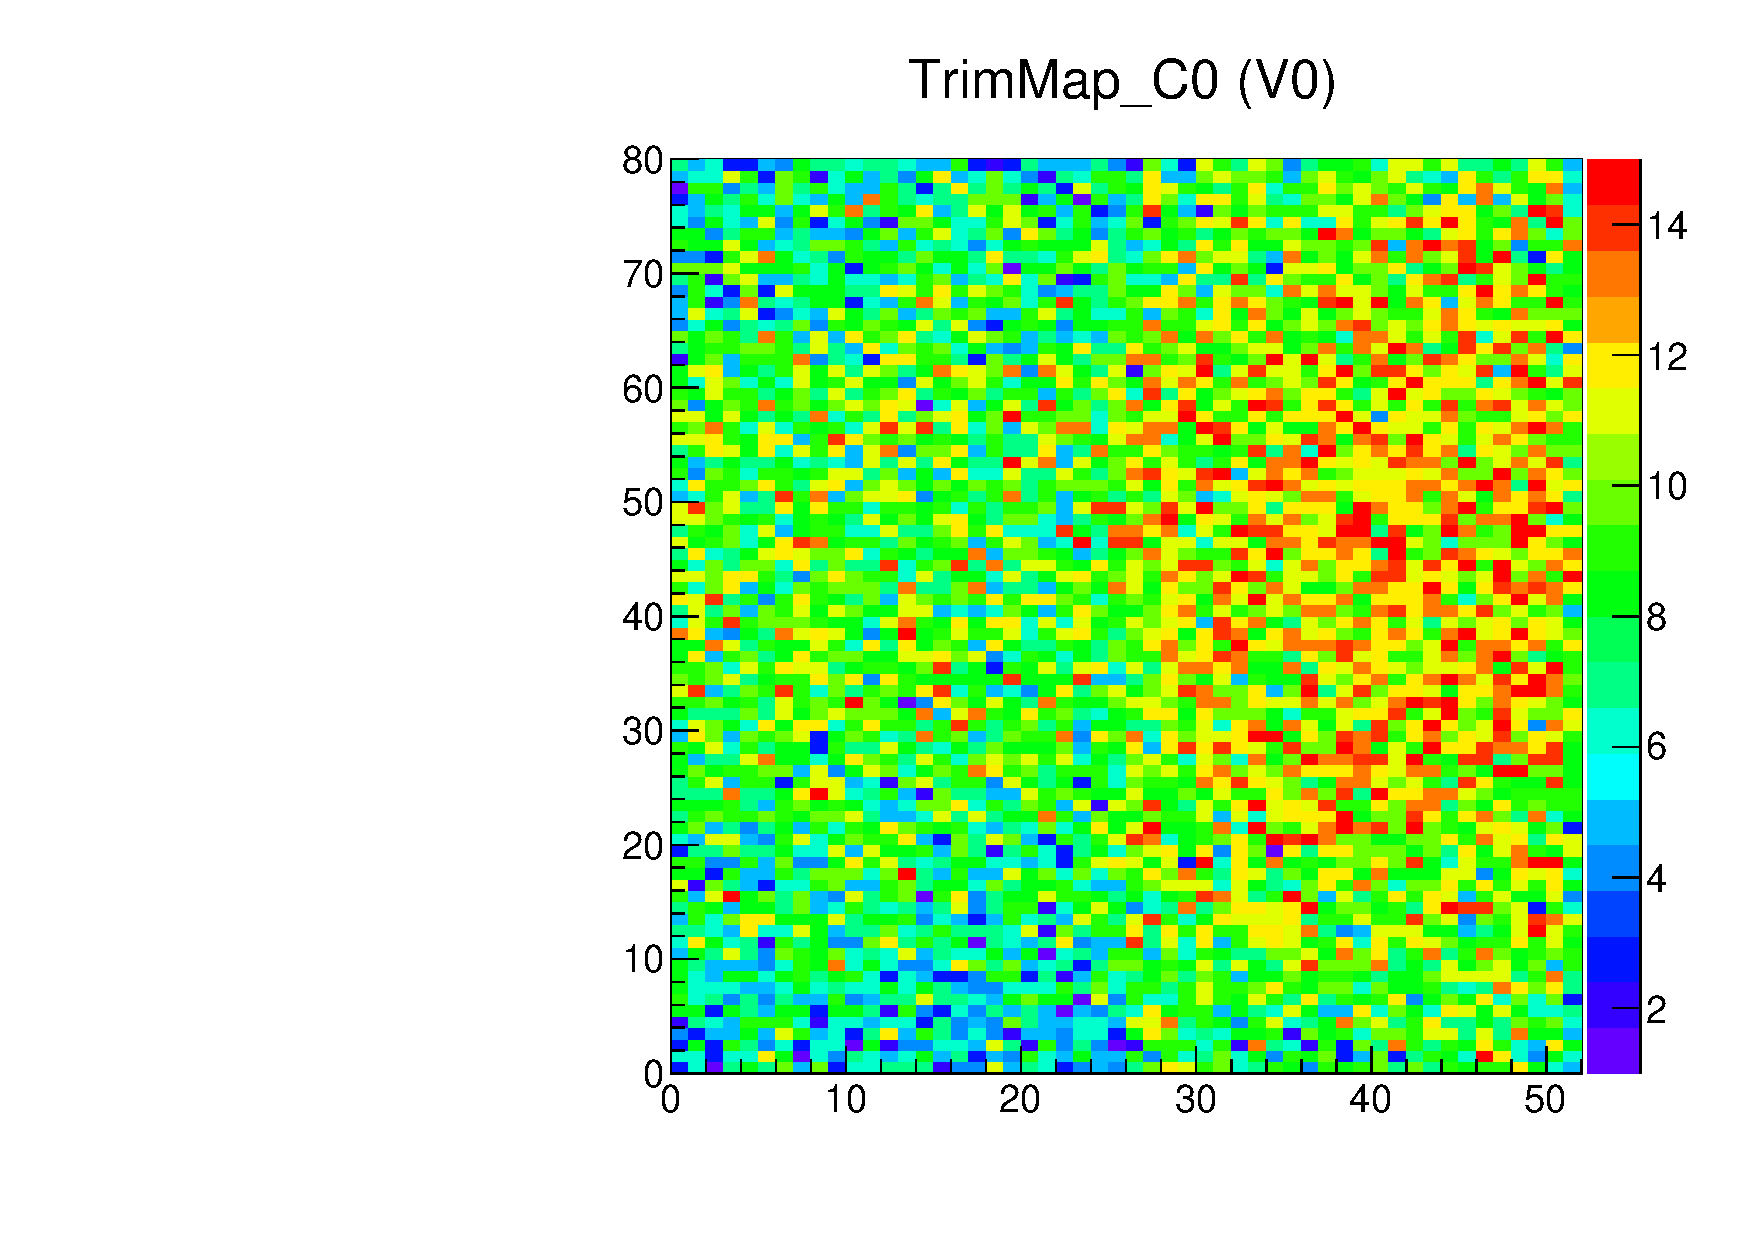
\includegraphics[width=1.0\textwidth]{figures/trim_TrimMap.pdf}
  \caption{\roc map of the optimized trim bit values (0-15).}
  \label{fig:trim_TrimMap}
\end{minipage}
\hspace{0.3cm}
\begin{minipage}{0.45\textwidth}
  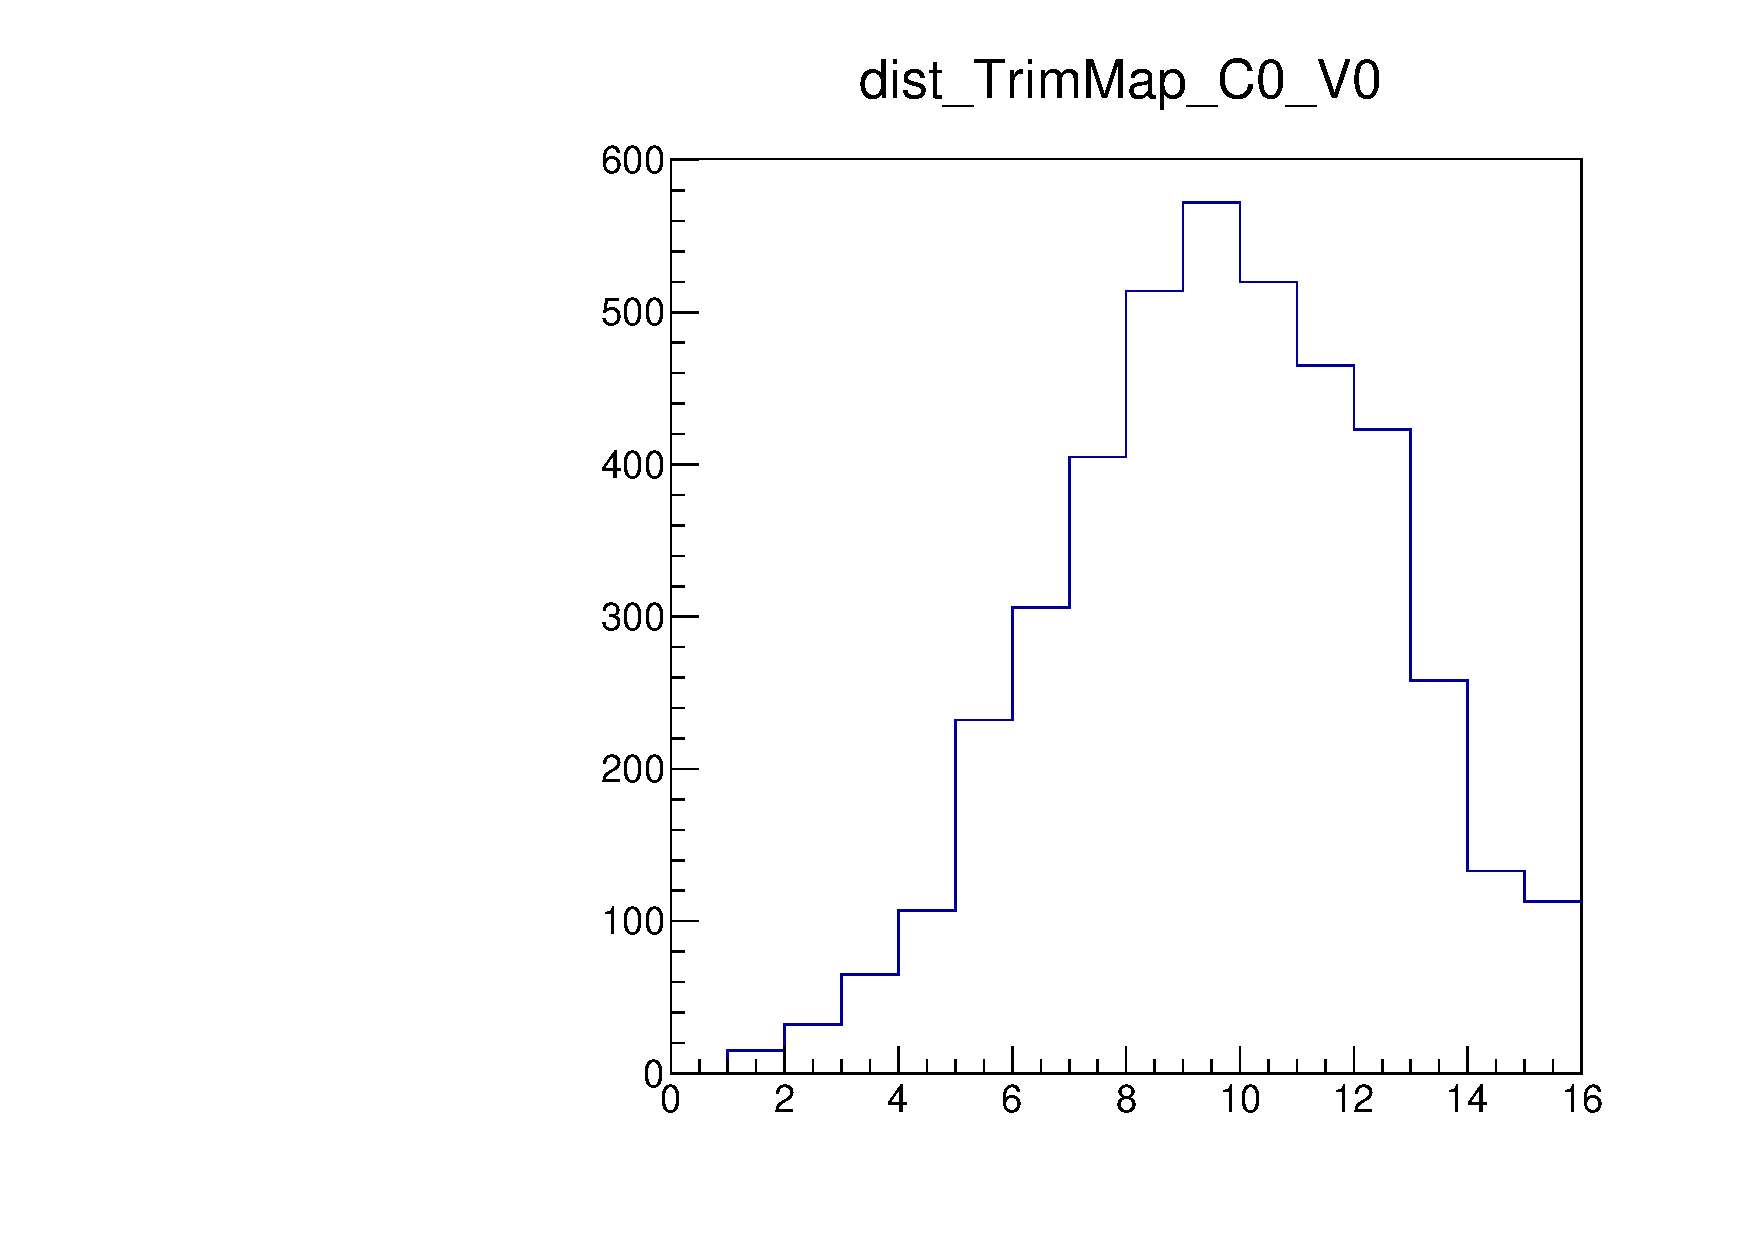
\includegraphics[width=1.0\textwidth]{figures/trim_dist_TrimMap.pdf}
  \caption{1D distribution of the optimized trim bit values (0-15).}
  \label{fig:trim_dist_TrimMap}
\end{minipage}
\end{figure}

% from trim test: vcal turn-on after trimming

\begin{figure}[!htp]
\centering
\begin{minipage}{0.45\textwidth}
  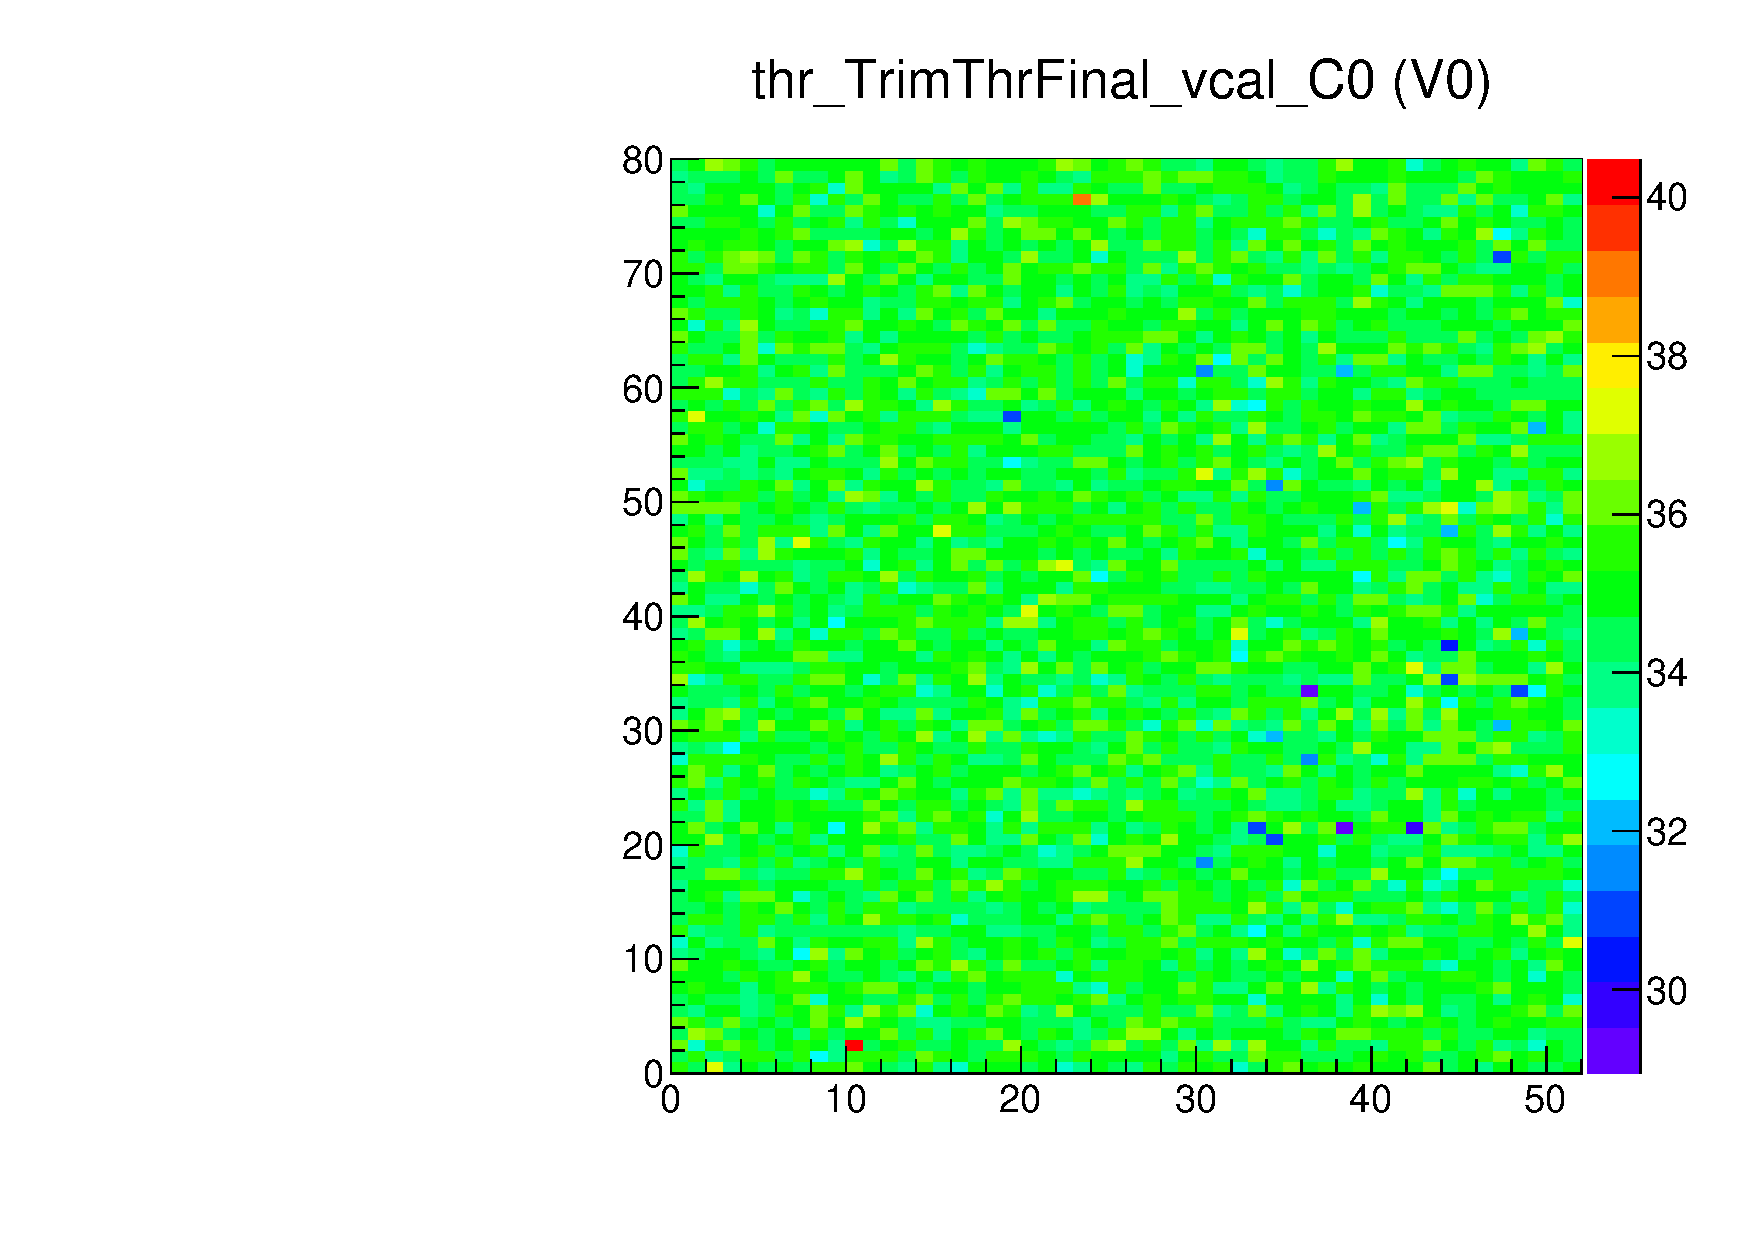
\includegraphics[width=1.0\textwidth]{figures/trim_thr_TrimThrFinal_vcal.pdf}
  \caption{\roc map of the \vcal turn-on thresholds with optimized trim parameters.}
  \label{fig:trim_thr_TrimThrFinal_vcal}
\end{minipage}
\hspace{0.3cm}
\begin{minipage}{0.45\textwidth}
  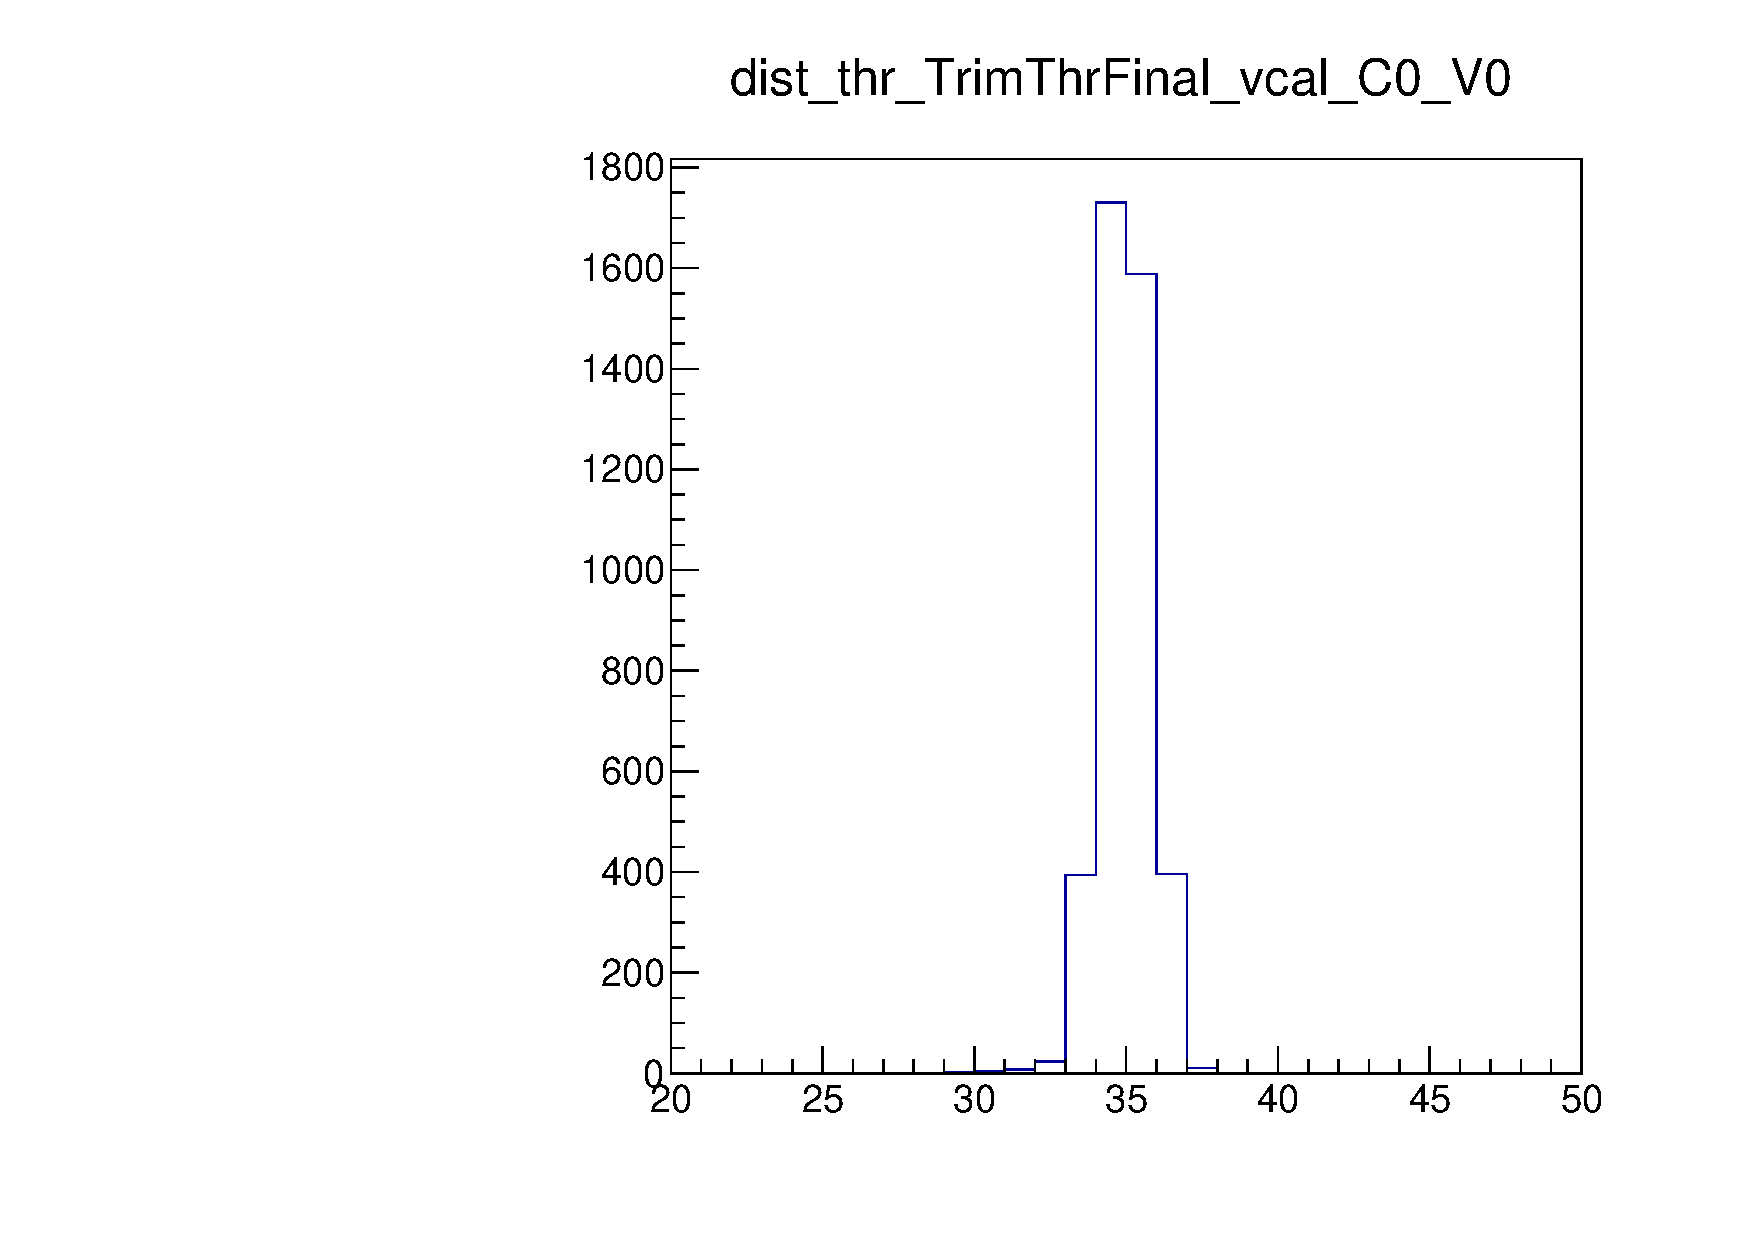
\includegraphics[width=1.0\textwidth]{figures/trim_dist_thr_TrimThrFinal_vcal.pdf}
  \caption{1D distribution of the \vcal turn-on thresholds with optimized trim parameters. [original range 0-255]}
  \label{fig:trim_dist_thr_TrimThrFinal_vcal}
\end{minipage}
\end{figure}


% ---------------------------------------------------------------------


% from trim bit test: untrimmed thresholds (trim bits = 15)

\begin{figure}[!htp]
\centering
\begin{minipage}{0.45\textwidth}
  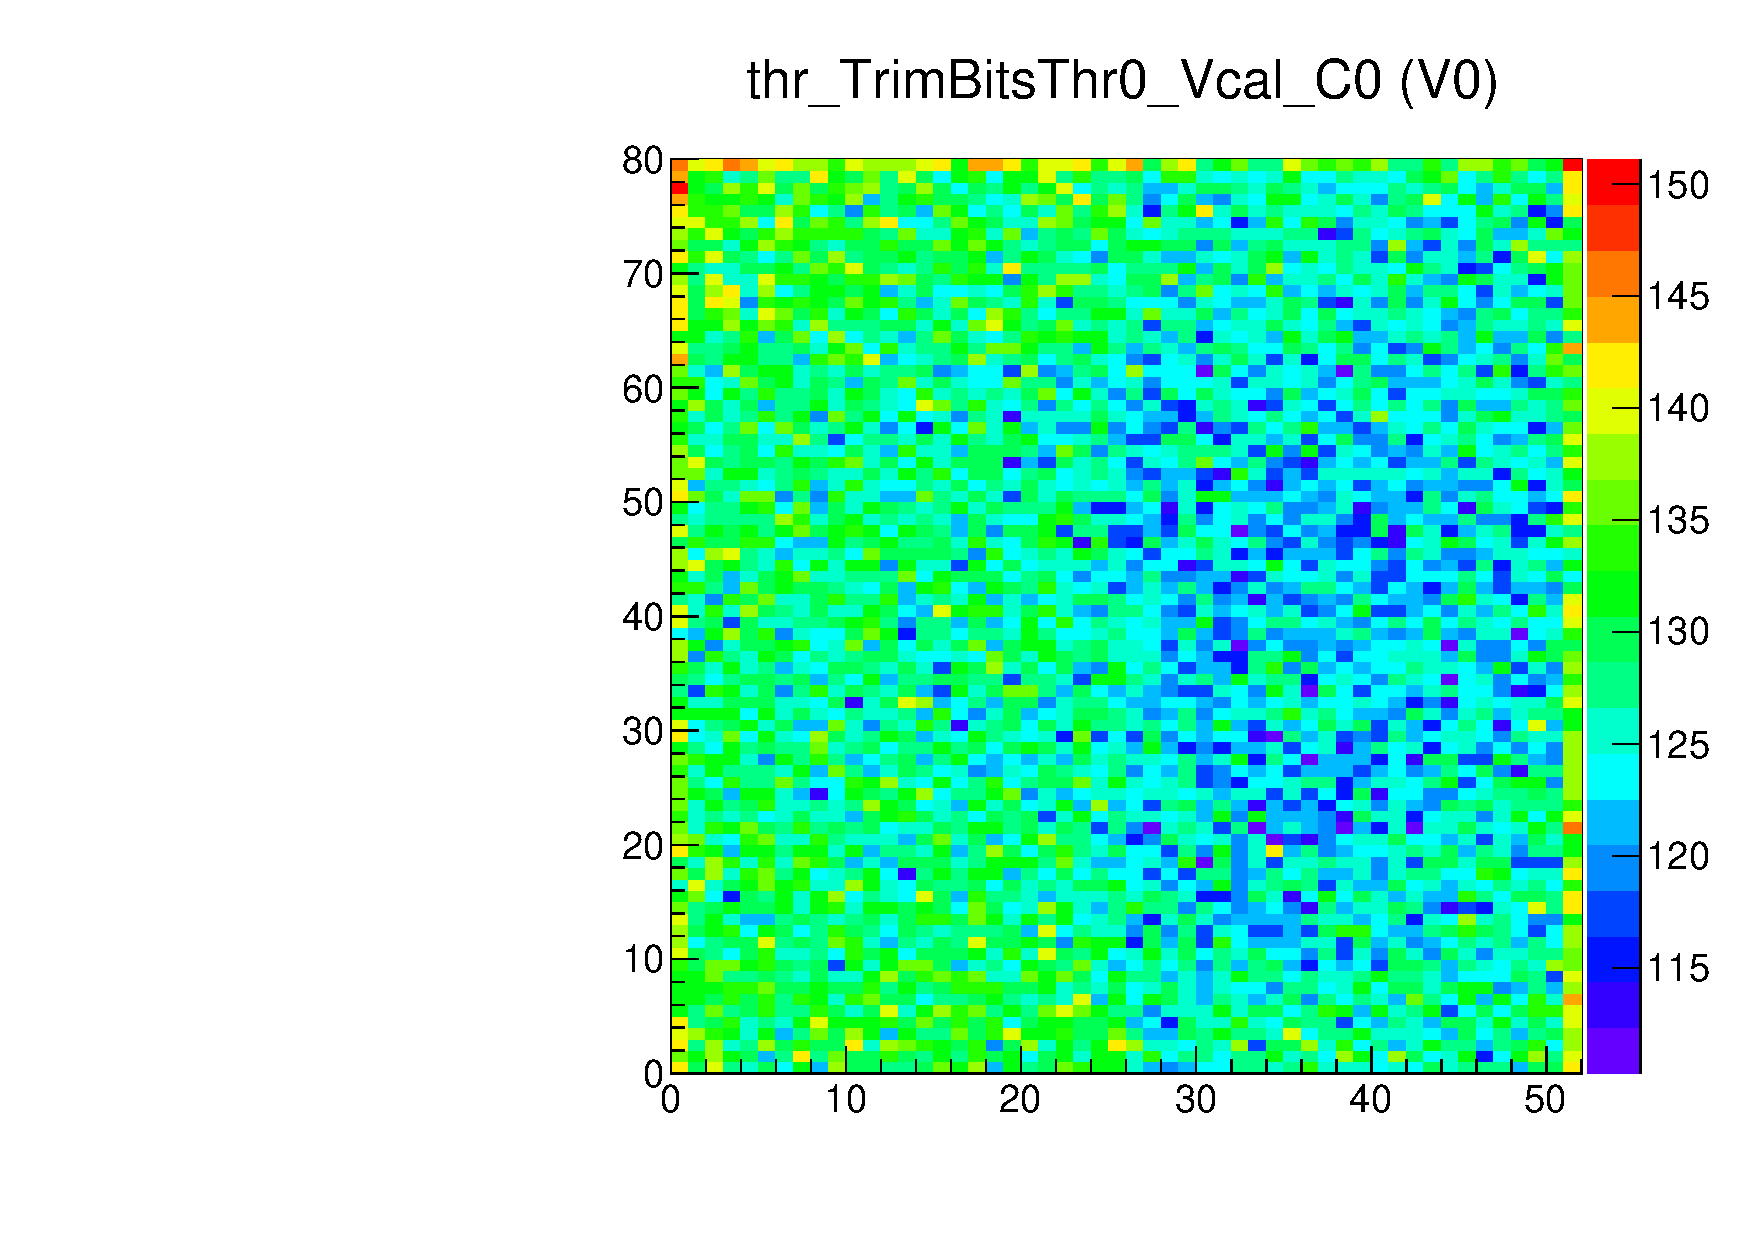
\includegraphics[width=1.0\textwidth]{figures/trim_thr_TrimBitsThr0_Vcal.pdf}
  \caption{\roc map of untrimmed \vcal thresholds.
           Used as a baseline for the \trimbit test.}
  \label{fig:trim_thr_TrimBitsThr0_Vcal}
\end{minipage}
\end{figure}


% from trim bits test:  vcal thresholds for different trim bit values trim_thr_TrimThr

\begin{figure}[!htp]
\centering
\begin{minipage}{0.45\textwidth}
  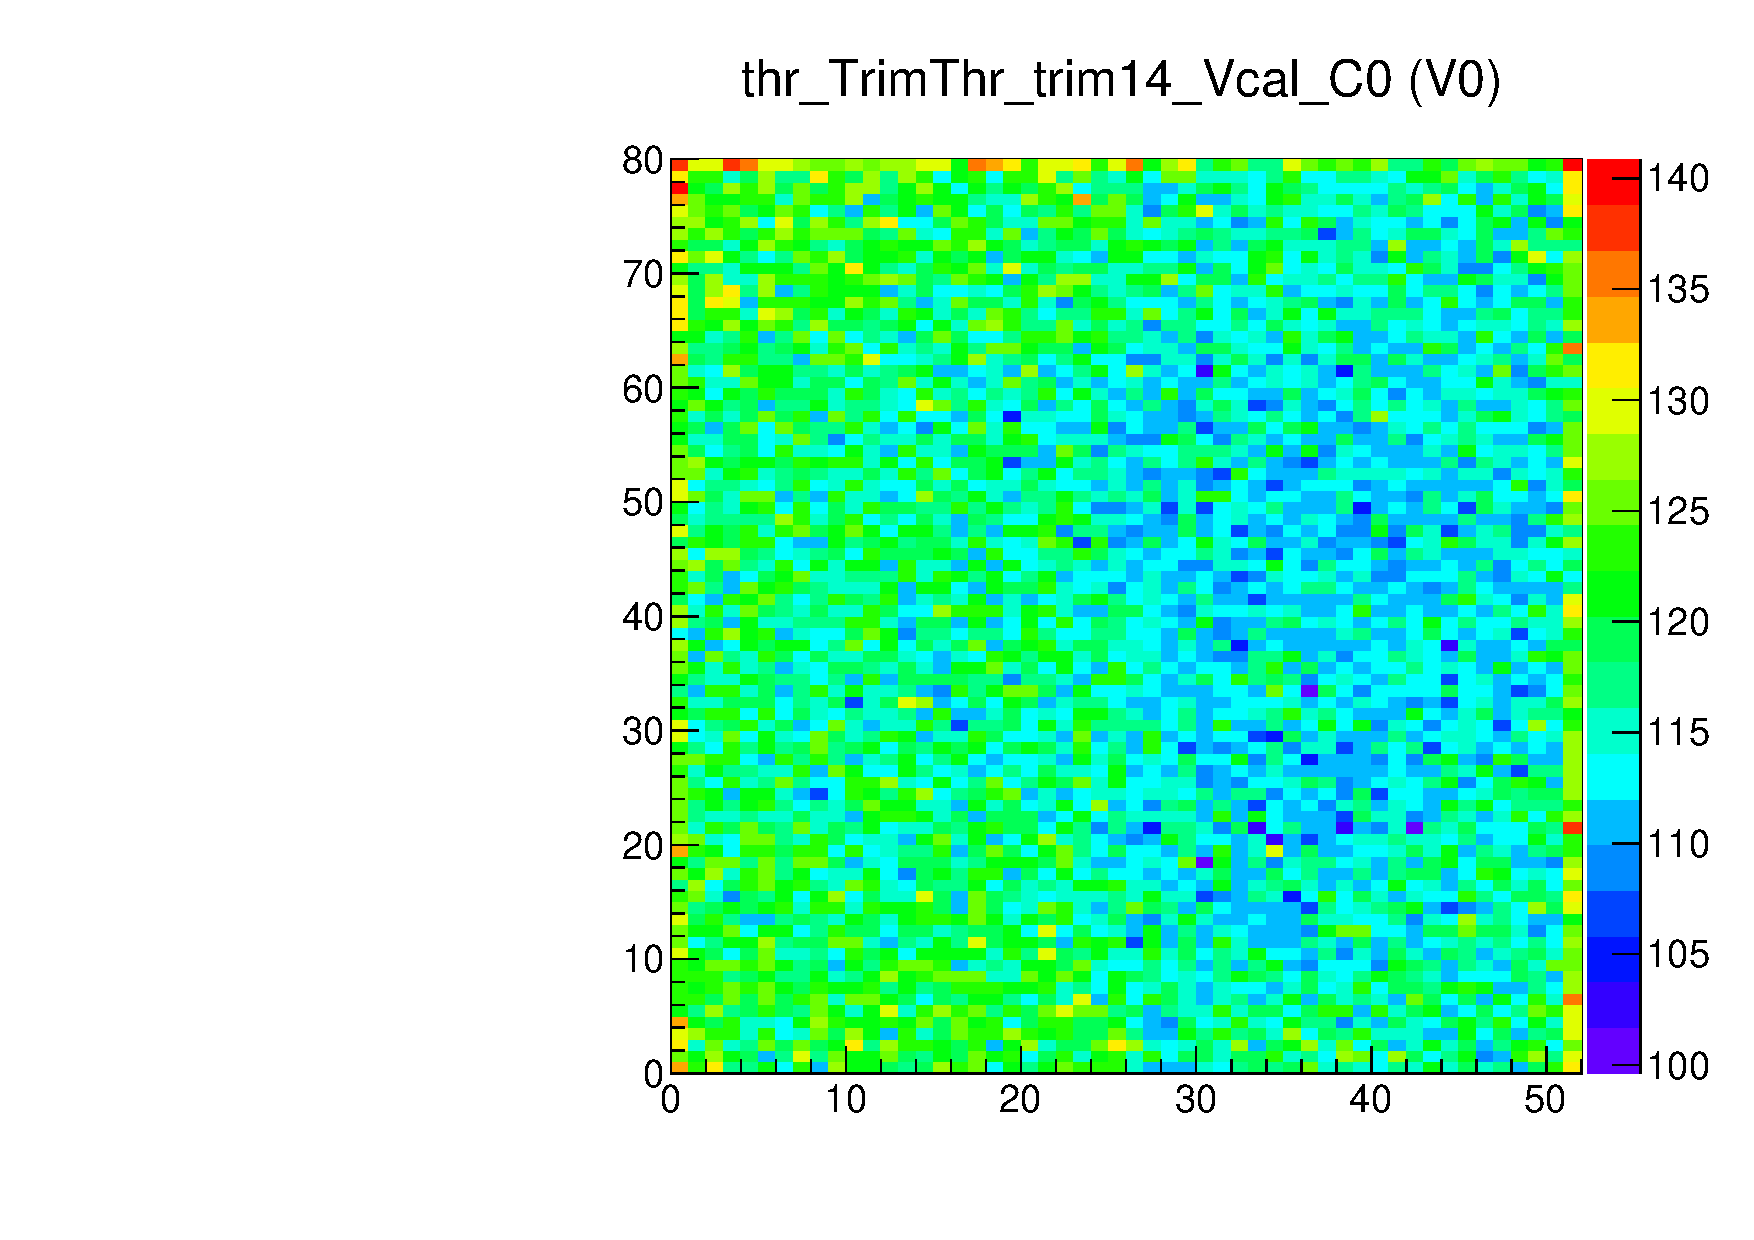
\includegraphics[width=1.0\textwidth]{figures/trim_thr_TrimThr_trim14_Vcal.pdf}
  \caption{\roc map of \vcal thresholds with \trimbits=14 [1110].}
  \label{fig:trim_thr_TrimThr_trim14_Vcal}
\end{minipage}
\hspace{0.3cm}
\begin{minipage}{0.45\textwidth}
  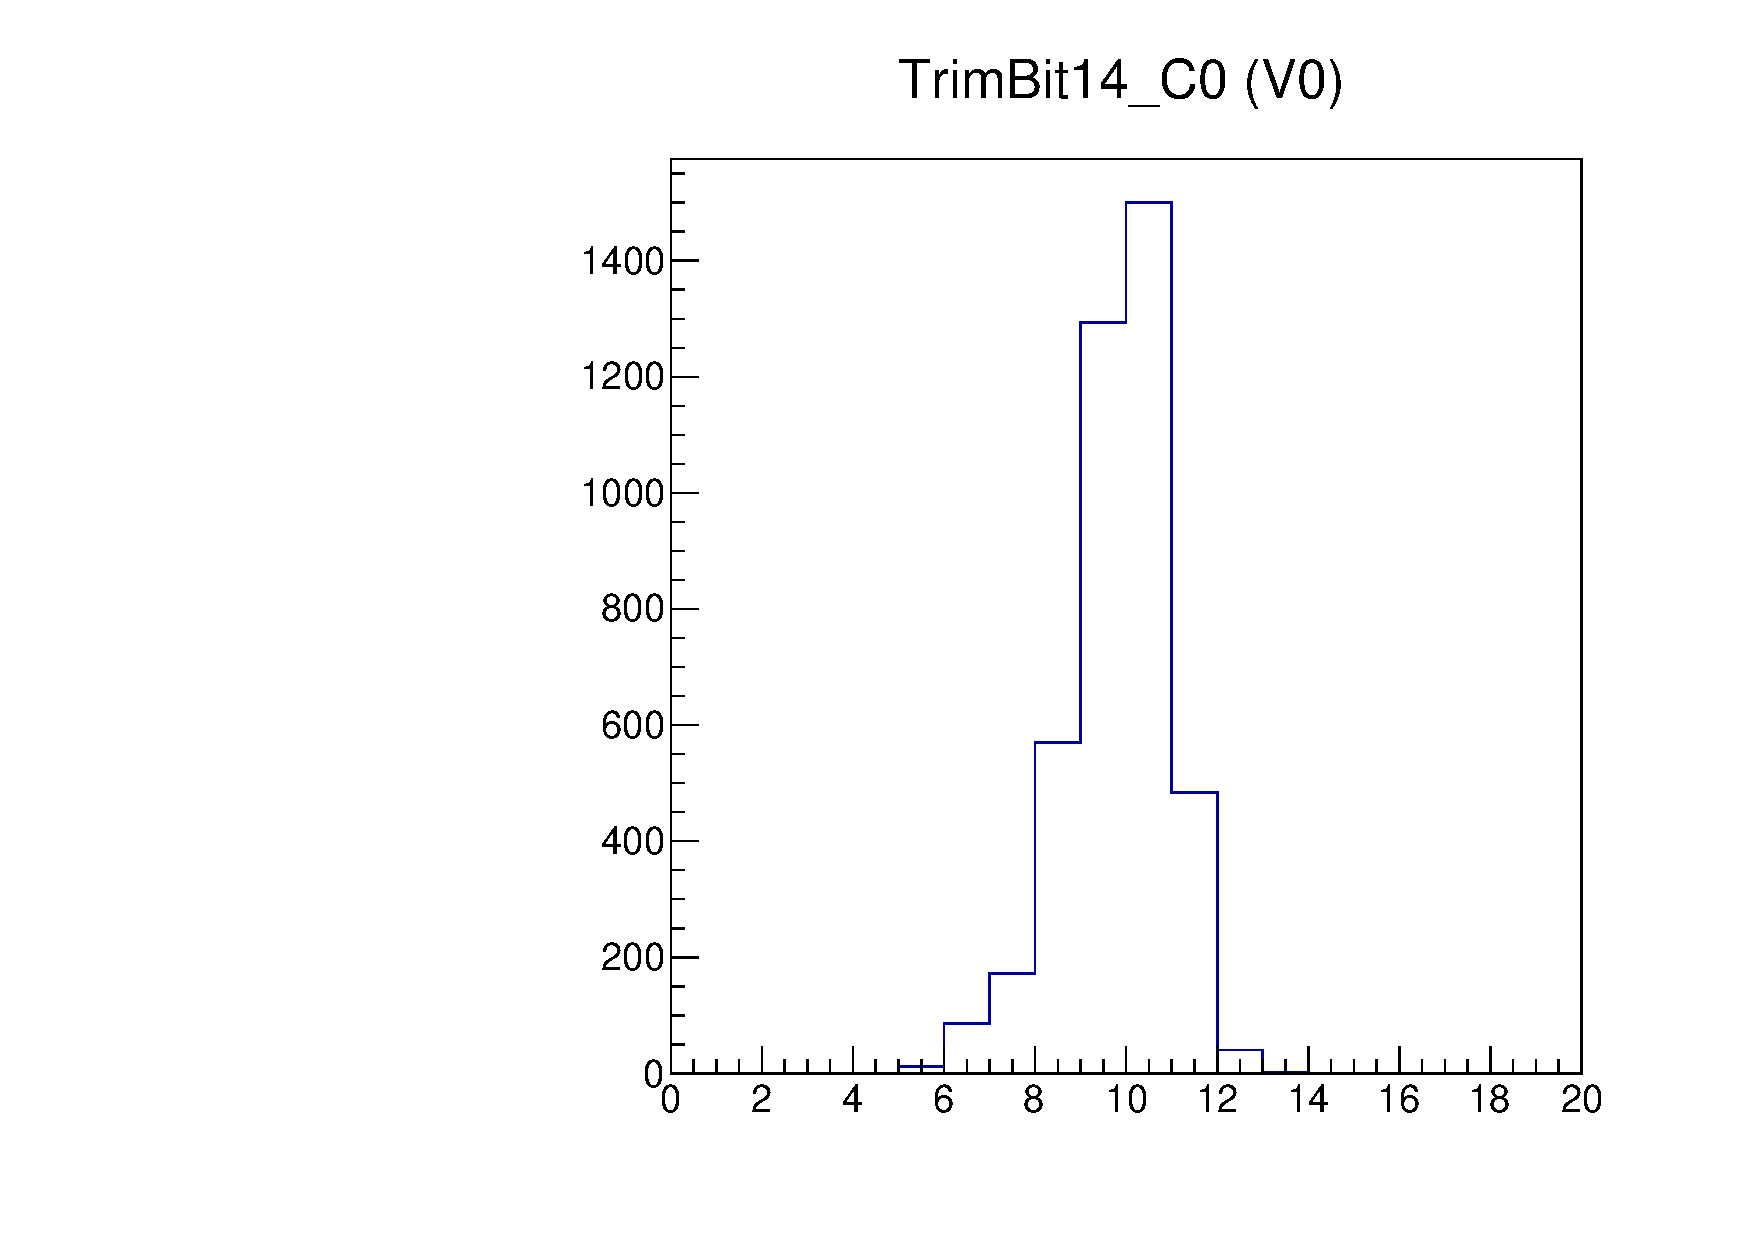
\includegraphics[width=1.0\textwidth]{figures/trim_TrimBit14.pdf}
  \caption{1D distribution of difference of Figure~\ref{fig:trim_thr_TrimBitsThr0_Vcal} and Figure~\ref{fig:trim_thr_TrimThr_trim14_Vcal}.
           Pixels with a faulty trim bit would populate the bin at zero.}
  \label{fig:trim_TrimBit14}
\end{minipage}
\end{figure}

\begin{figure}[!htp]
\centering
\begin{minipage}{0.45\textwidth}
  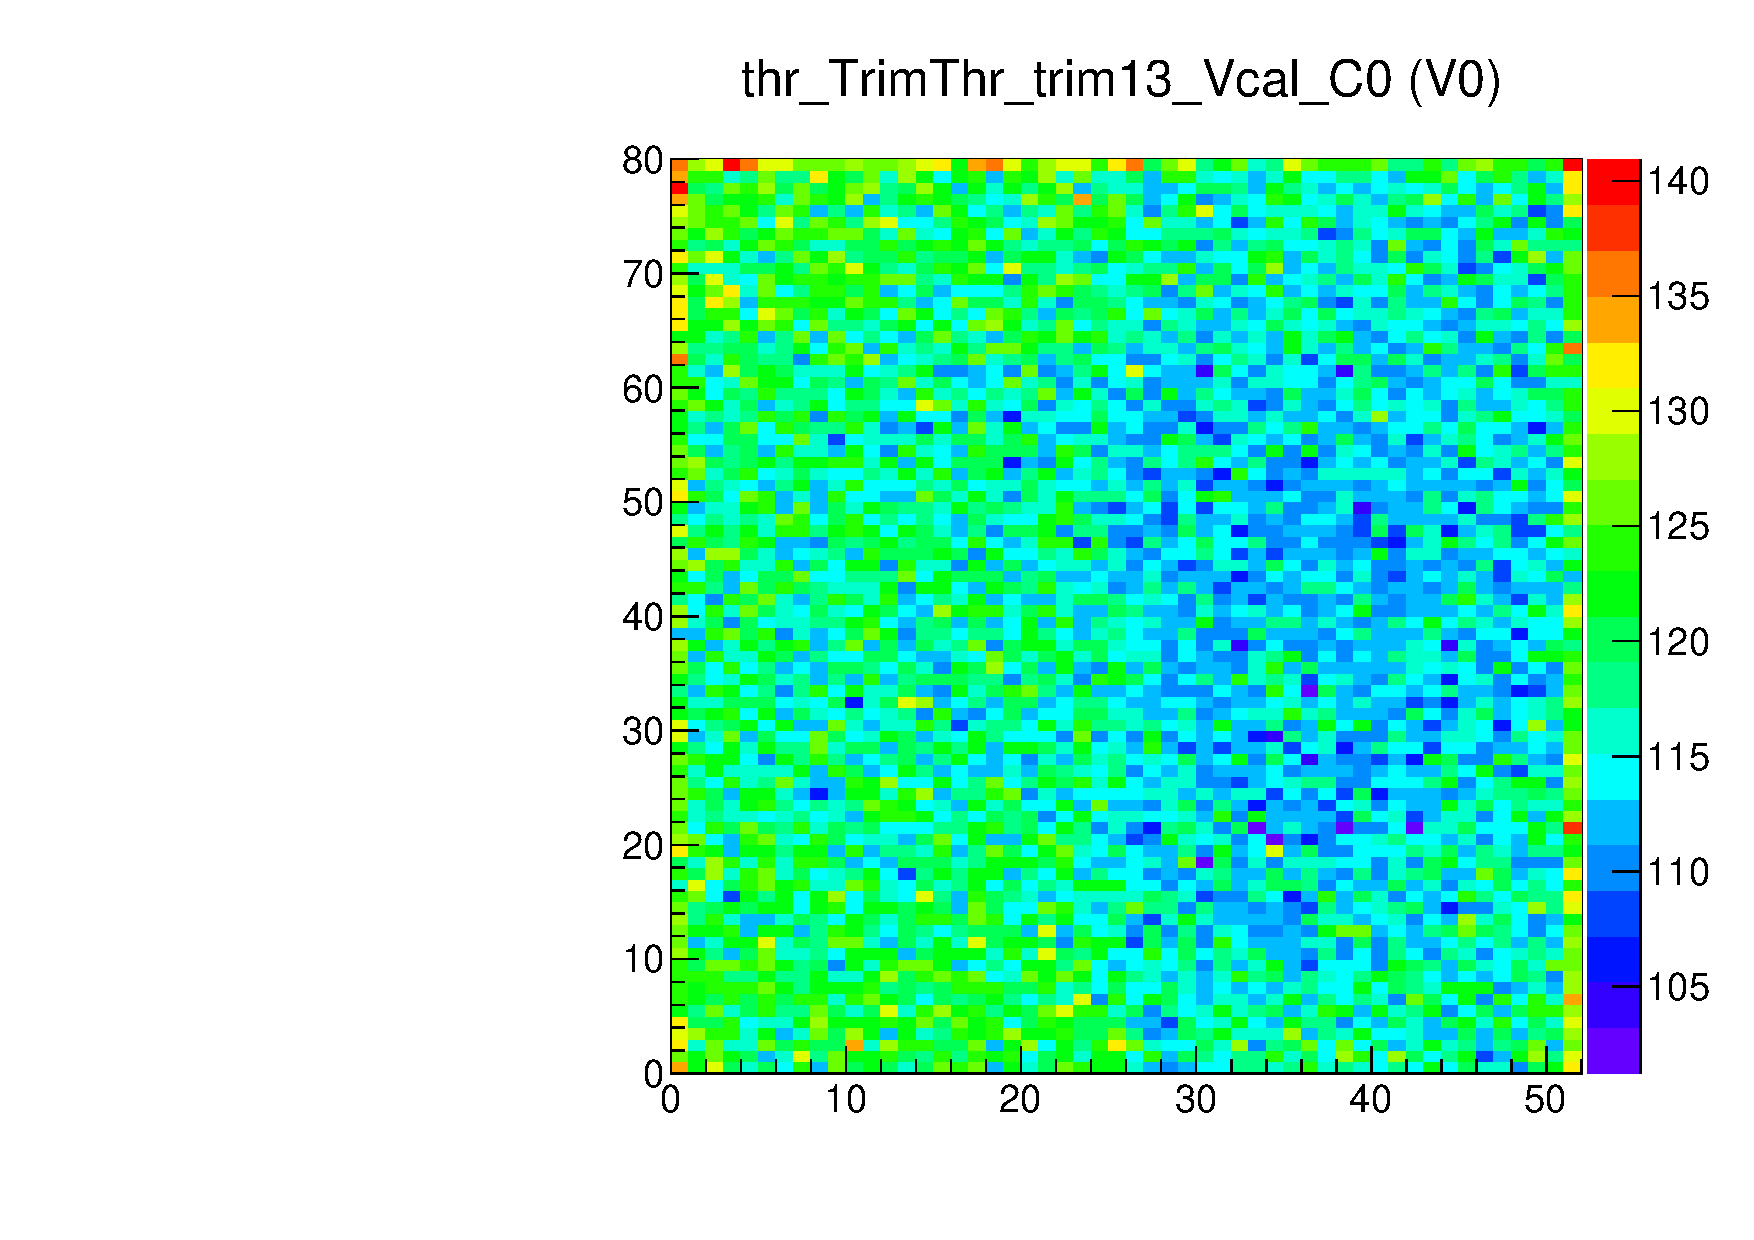
\includegraphics[width=1.0\textwidth]{figures/trim_thr_TrimThr_trim13_Vcal.pdf}
  \caption{\roc map of \vcal thresholds with \trimbits=13 [1101].}
  \label{fig:trim_thr_TrimThr_trim13_Vcal}
\end{minipage}
\hspace{0.3cm}
\begin{minipage}{0.45\textwidth}
  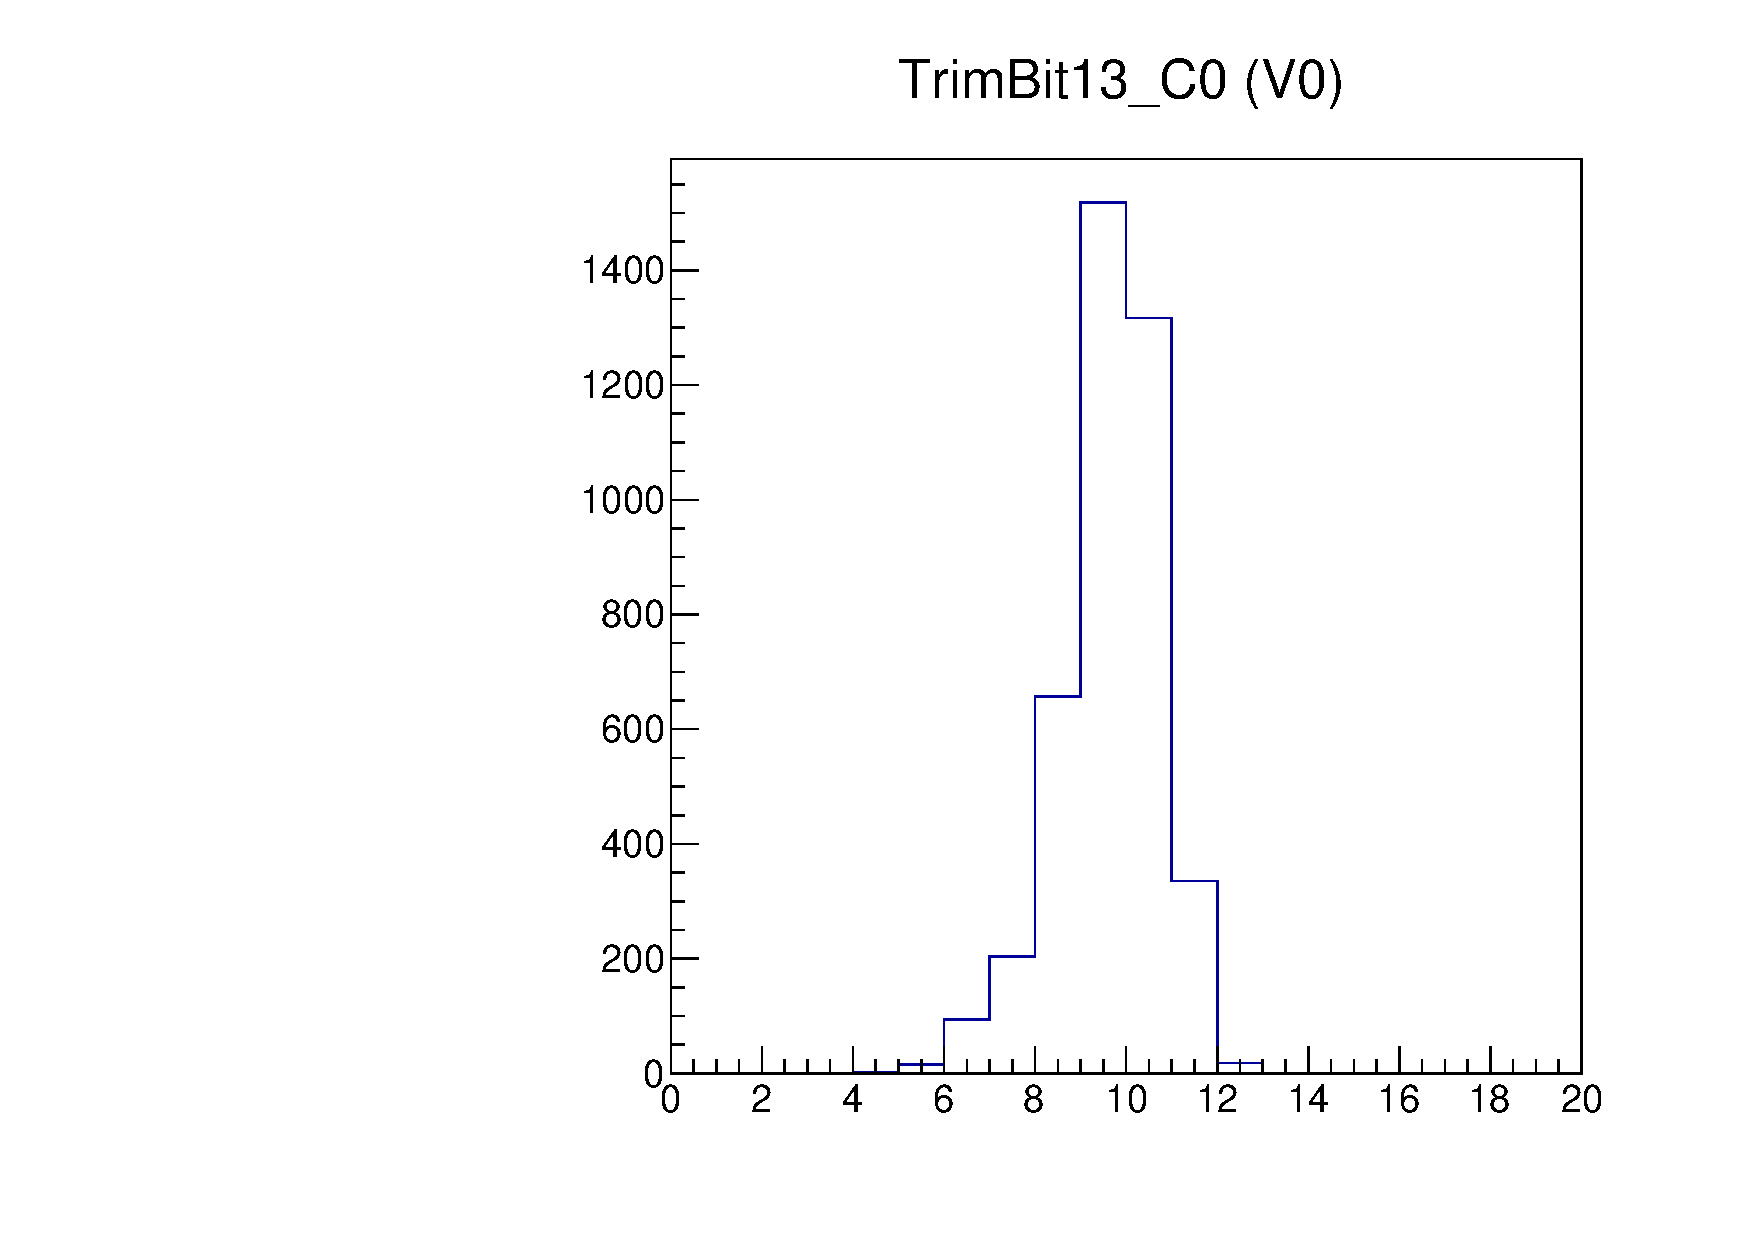
\includegraphics[width=1.0\textwidth]{figures/trim_TrimBit13.pdf}
  \caption{1D distribution of difference of Figure~\ref{fig:trim_thr_TrimBitsThr0_Vcal} and Figure~\ref{fig:trim_thr_TrimThr_trim13_Vcal}.
           Pixels with a faulty trim bit would populate the bin at zero.}
  \label{fig:trim_TrimBit13}
\end{minipage}
\end{figure}

\begin{figure}[!htp]
\centering
\begin{minipage}{0.45\textwidth}
  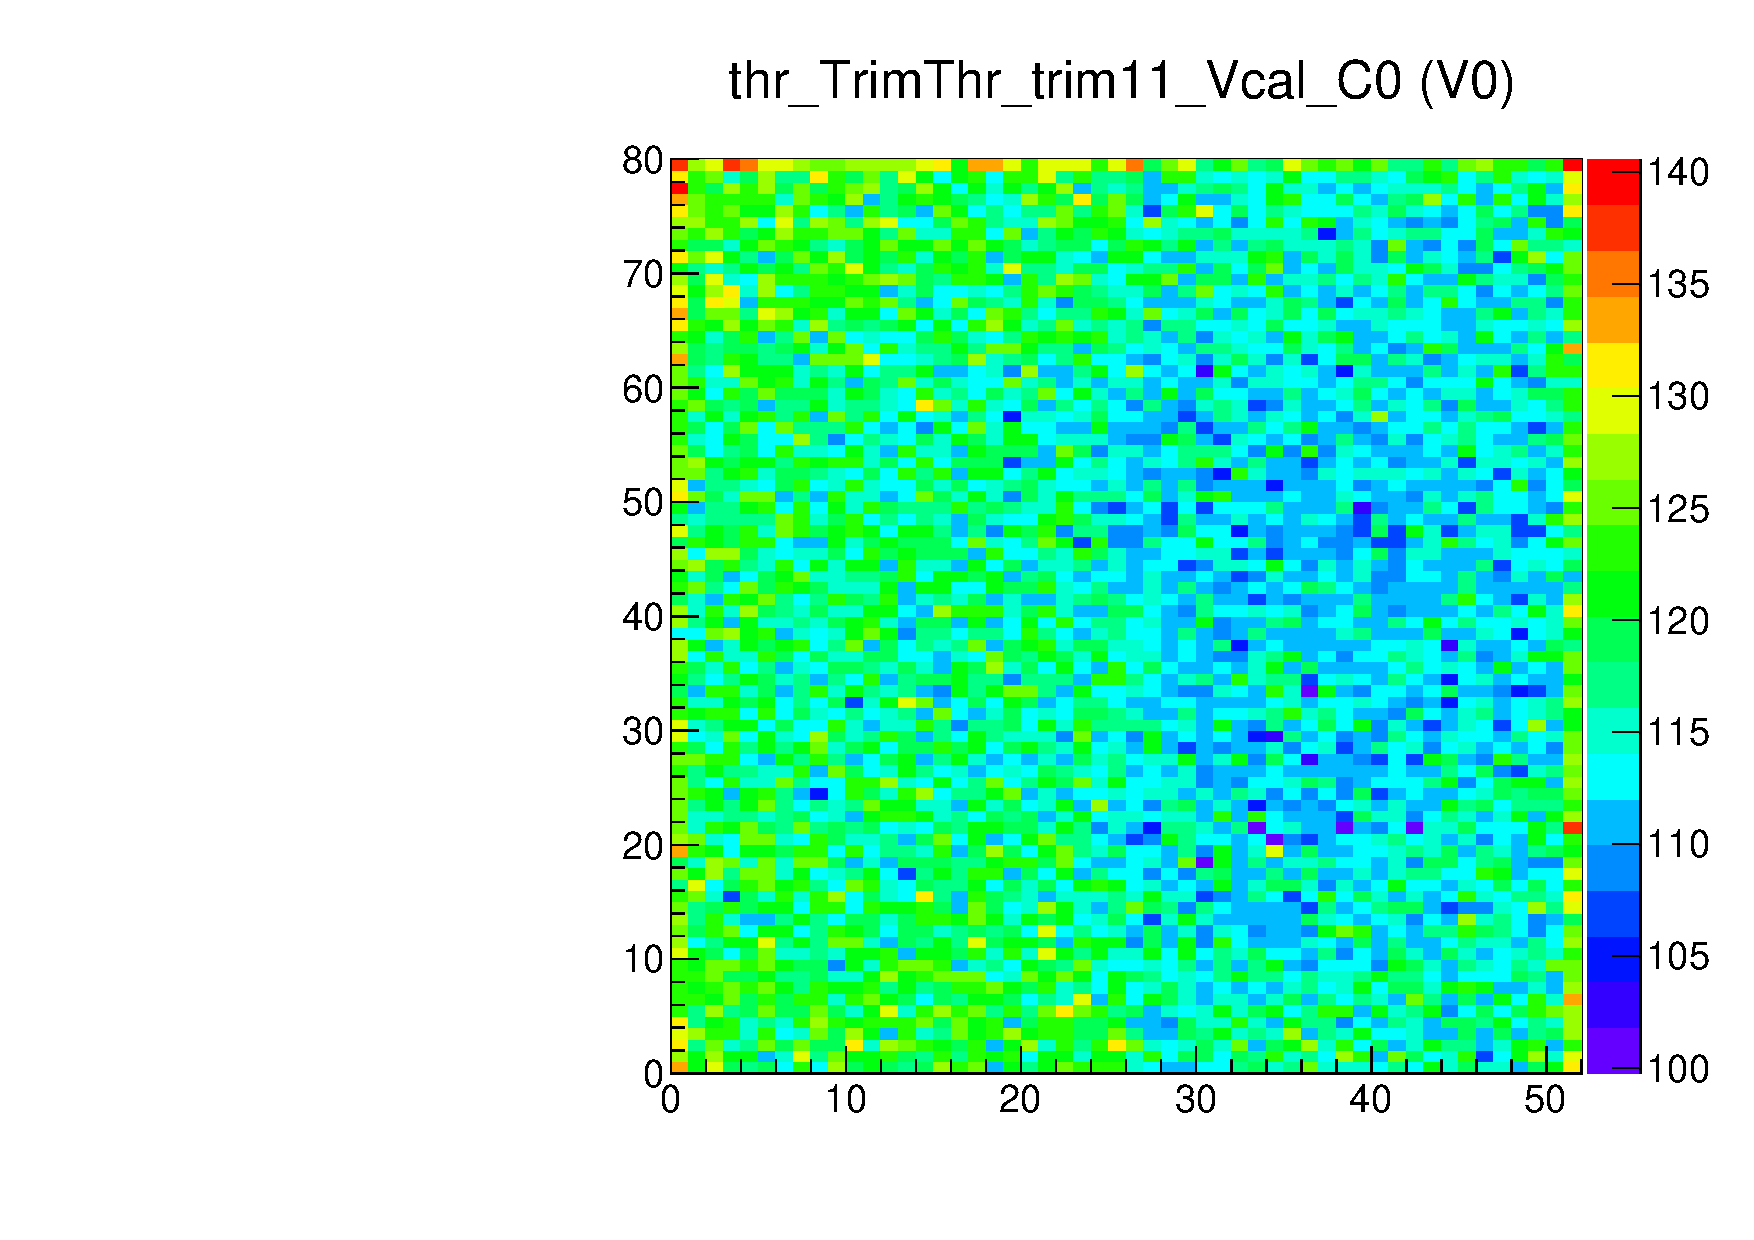
\includegraphics[width=1.0\textwidth]{figures/trim_thr_TrimThr_trim11_Vcal.pdf}
  \caption{\roc map of \vcal thresholds with \trimbits=11 [1011].}
  \label{fig:trim_thr_TrimThr_trim11_Vcal}
\end{minipage}
\hspace{0.3cm}
\begin{minipage}{0.45\textwidth}
  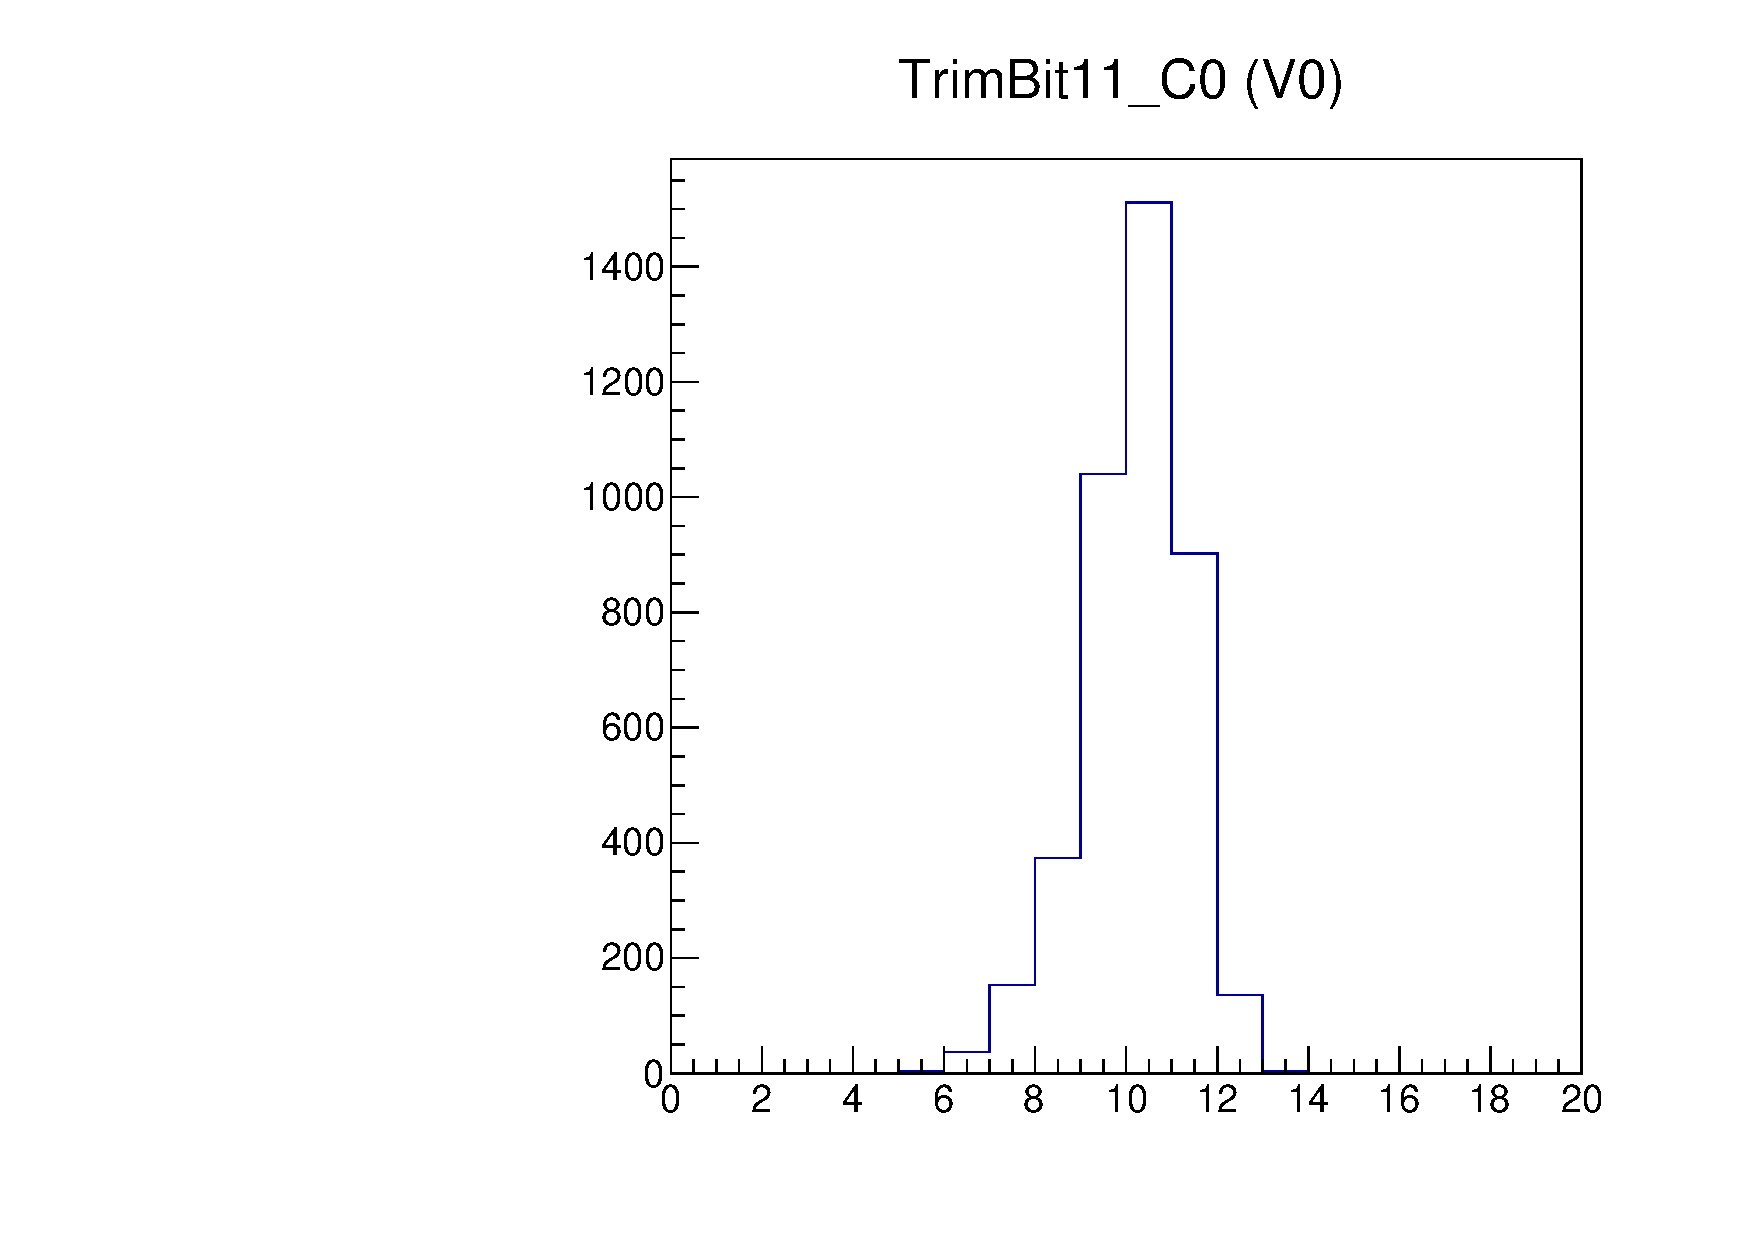
\includegraphics[width=1.0\textwidth]{figures/trim_TrimBit11.pdf}
  \caption{1D distribution of difference of Figure~\ref{fig:trim_thr_TrimBitsThr0_Vcal} and Figure~\ref{fig:trim_thr_TrimThr_trim11_Vcal}.
           Pixels with a faulty trim bit would populate the bin at zero.}
  \label{fig:trim_TrimBit11}
\end{minipage}
\end{figure}

\begin{figure}[!htp]
\centering
\begin{minipage}{0.45\textwidth}
  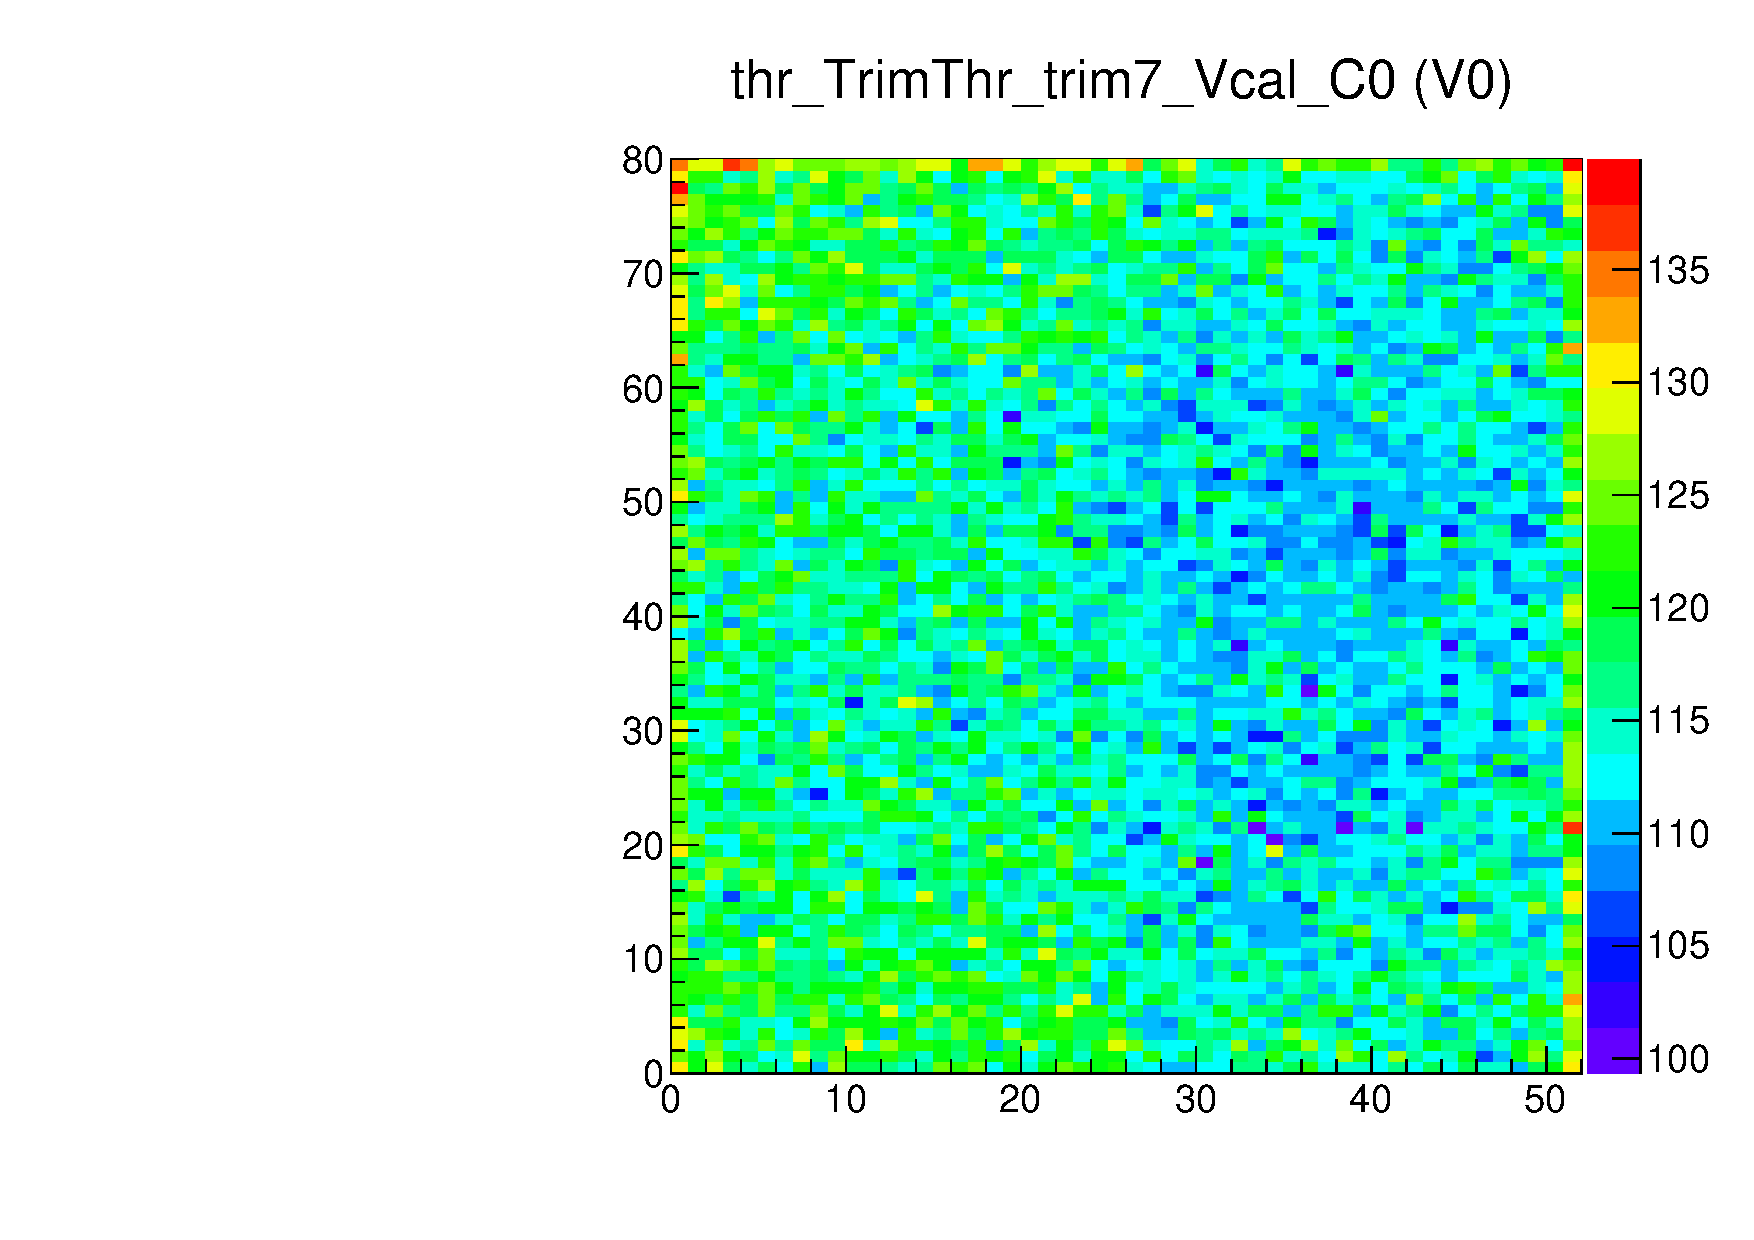
\includegraphics[width=1.0\textwidth]{figures/trim_thr_TrimThr_trim7_Vcal.pdf}
  \caption{\roc map of \vcal thresholds with \trimbits=7 [0111].}
  \label{fig:trim_thr_TrimThr_trim7_Vcal}
\end{minipage}
\hspace{0.3cm}
\begin{minipage}{0.45\textwidth}
  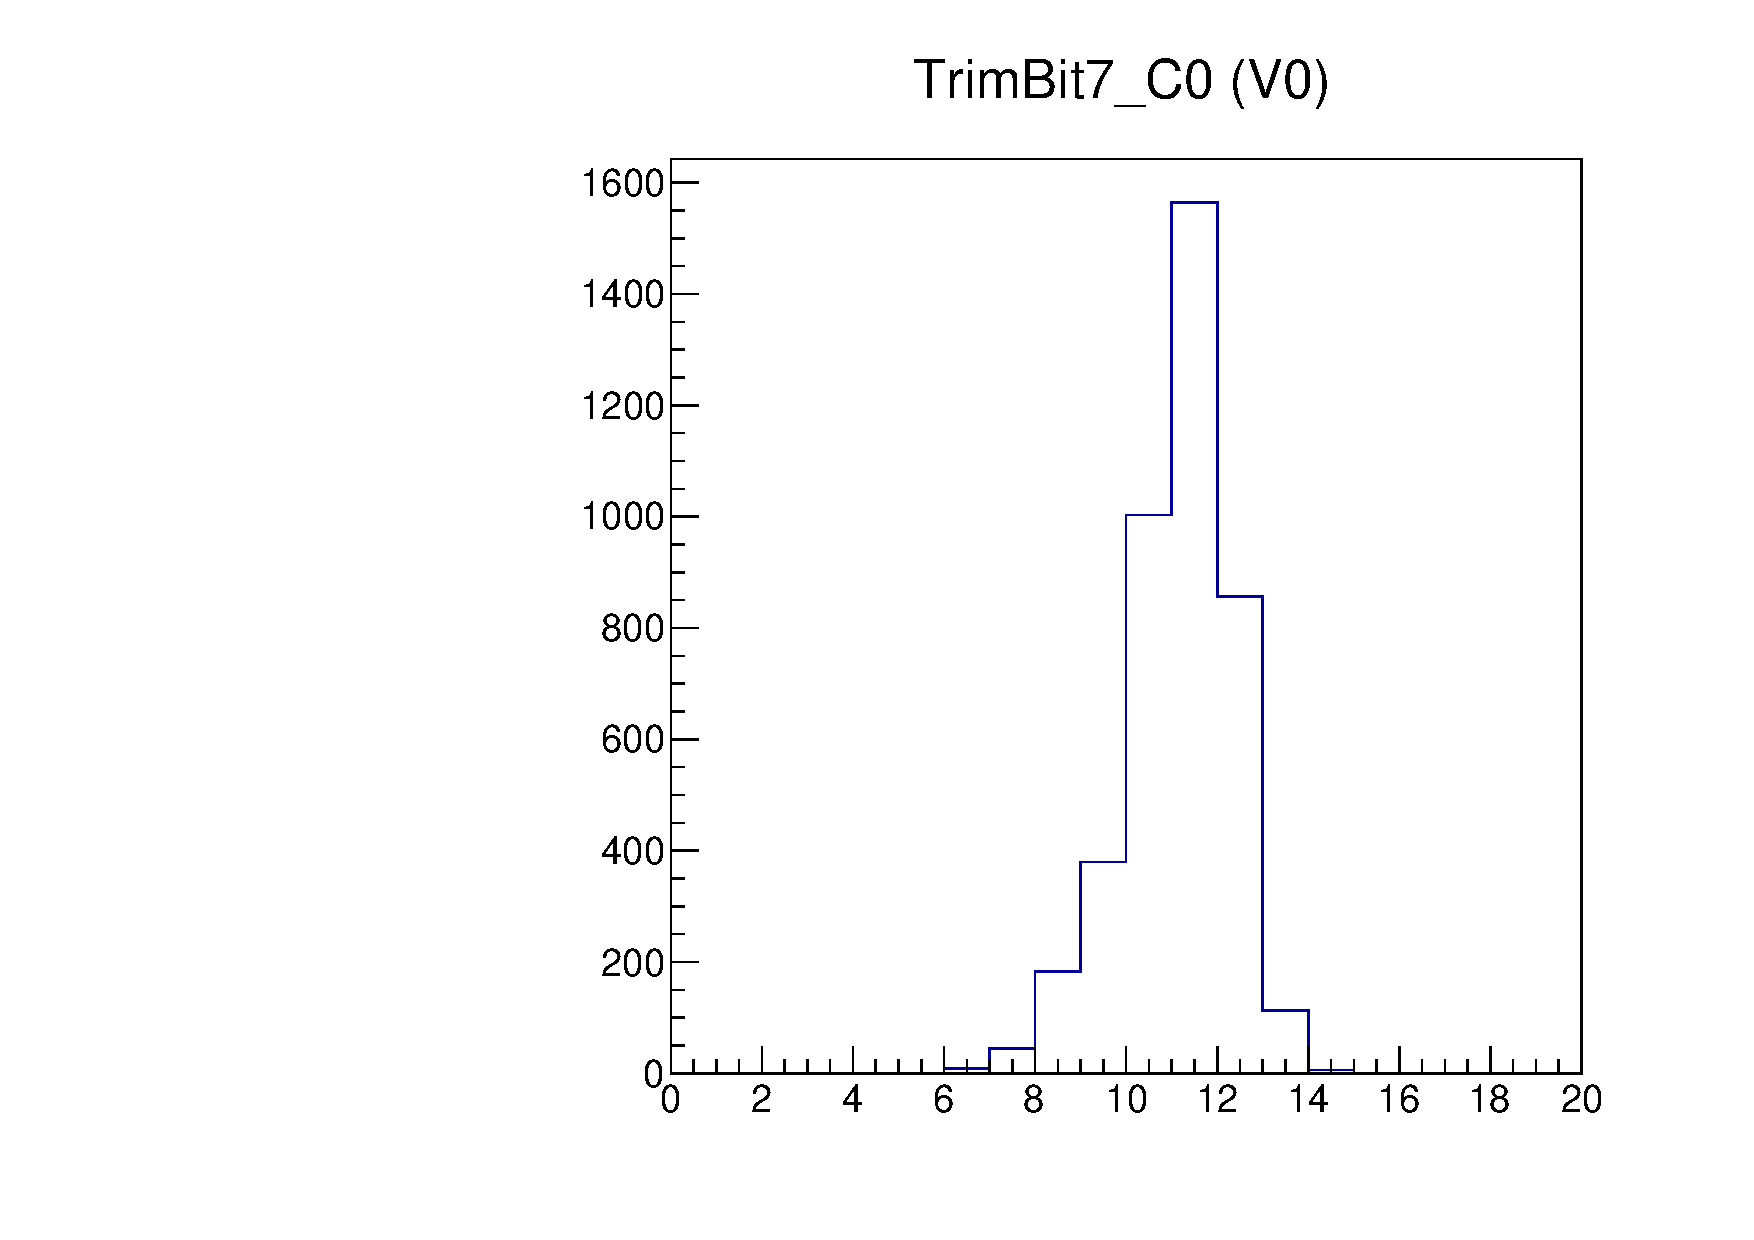
\includegraphics[width=1.0\textwidth]{figures/trim_TrimBit7.pdf}
  \caption{1D distribution of difference of Figure~\ref{fig:trim_thr_TrimBitsThr0_Vcal} and Figure~\ref{fig:trim_thr_TrimThr_trim7_Vcal}.
           Pixels with a faulty trim bit would populate the bin at zero.}
  \label{fig:trim_TrimBit7}
\end{minipage}
\end{figure}

